%% Intended to be included into a larger document
\chapter{Related Work}
\label{cha:related-work}

This chapter examines research related to sustainability, serious games and gamification, game design, serious game frameworks, and framework assessment. \autoref{sec:rel-sustainability} and \autoref{sec:rel-competition} discusses the needs for sustainability education and the current implementation of collegiate sustainability competitions. \autoref{sec:rel-seriousgame} discusses related work on serious games and recent development in gamification. \autoref{sec:rel-sg-sustainability} looks at the applications of ``serious game'' in the sustainability context. Finally, \autoref{sec:rel-sg-framework} and \autoref{sec:rel-sg-assessment} examine the serious game framework and its assessment.

\section{Sustainability and Education}
\label{sec:rel-sustainability}

Sustainability is defined as ``a requirement of our generation to manage the
resource base such that the average quality of life that we ensure ourselves can potentially
be shared by all future generations''\cite{asheim1994sustainability}. The depletion of natural
resource has become a major focus of governments, organizations and citizens all over the world. 
There is widespread support for a dramatic increase in energy efficiency and change in
energy use from fossil fuels to renewable sources\cite{lenssen1996sustainable}. 

In Hawaii, the need for transition is especially acute, as the
state leads the US both in the price of energy and reliance on fossil fuels as an 
energy source. Almost 90\% of the energy used in Hawaii is from imported fossil fuel, primarily oil, \cite{hawaiienergypolicy}, as shown in \autoref{fig:hawaii-energy}. Launched by the US Department of Energy and the State of Hawaii, the Hawaii Clean Energy Initiative \cite{hcei} aims to achieve 70\% clean energy by 2030 with 30\% from efficiency measures, and 40\% coming from locally generated renewable sources.

\begin{figure}[ht!]
	\centering
		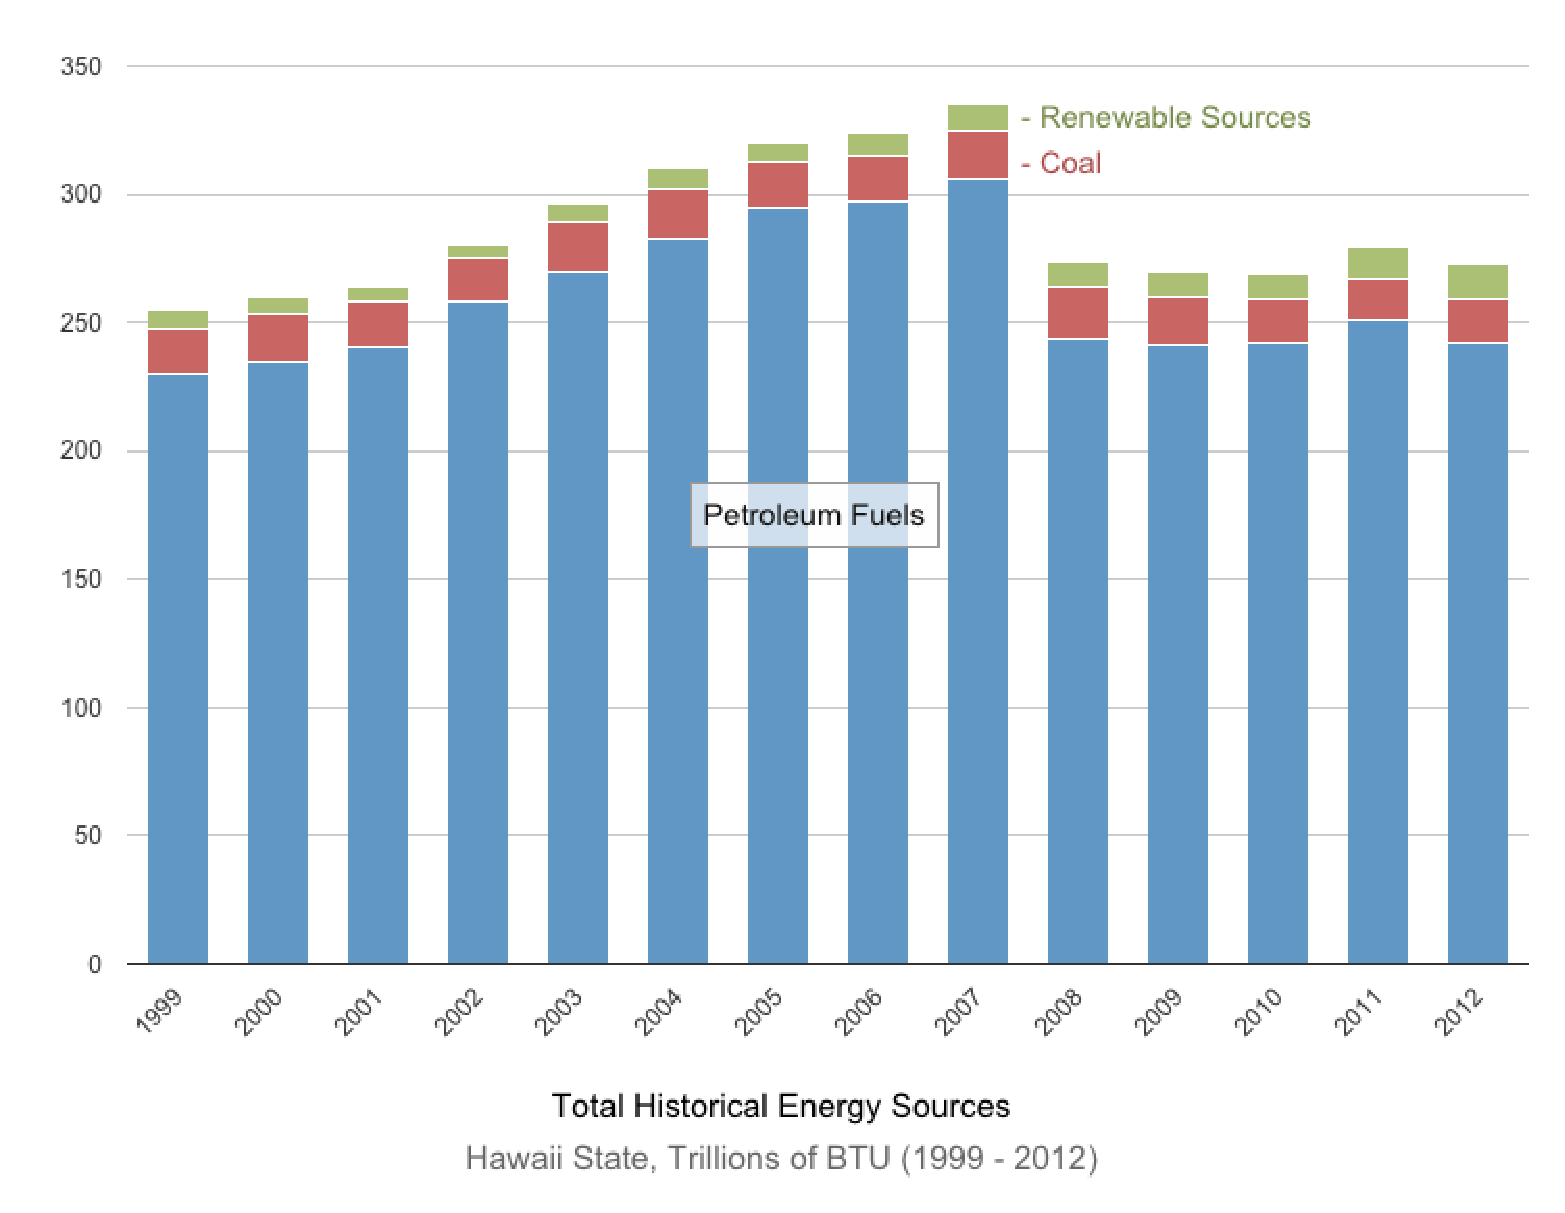
\includegraphics[width=0.6\columnwidth]{hawaii-energy}
		\caption{ Hawaii Energy Sources \cite {hawaiienergypolicy}} 
		\label{fig:hawaii-energy}
\end{figure}

Government action is required to change the balance between methods of generation and consumption. On the other hand, in terms of personal change for a sustainable lifestyle, ``green'' actions addressing responsibility as consumers such as recycling, and saving energy and water need to be pursued \cite{kagawa2007dissonance}.  

changing people's behavior with respect to energy holds significant promise in reducing energy use. Darby's survey of energy consumption research found that identical homes could differ in energy use by a factor of two or more \cite{darby-review-2006}. Data from a military housing community on Oahu show energy usage for similar homes can differ by a factor of 4 \cite{Norton2010ZeroEnergyHomes}.

\section{Collegiate Sustainability Competitions}
\label{sec:rel-competition}

The creation of Makahiki is largely motivated from the needs from colleges and universities in running sustainability competitions for for sustainability education. Energy and water competitions or challenges have been introduced to college dormitories and residential homes as ways to facilitate and incentivize resource reduction to achieve sustainability goals. A survey by Hodge found that there are 163 college residence hall energy competitions taking place or being planned for the 2010--2011 academic year in North America~\cite{Hodge2010} to engaging students in sustainability issues. Hodge found that the average reduction in electricity use during these competitions is 9\%. 

A basic type of sustainability competition use a ``minimal tech'' solution such as a web page and manual posting of data and results on a periodic basis such as weekly. The Harvard University Green Cup Competition \cite{harvard-green-cup} and the Wellesley College Green Cup \cite{wellesley-green-cup} are examples of this type of competition. During the 2012 Harvard University Green Cup Competition, there were 4.3\% electricity reduction across the participating residence houses and an individual house reduction of 16.6\%, as shown in \autoref{fig:greencup}.

\begin{figure}[ht!]
	\centering
		
\includegraphics[width=0.6\columnwidth]{harvard-green-cup}
		\caption{Harvard Green Cup Competition for Energy}
		\label{fig:greencup}
\end{figure}

Some organizations built their own custom in-house solutions to support the infrastructure need for sustainability competitions. Oberlin College dorm energy competition \cite{petersen-dorm-energy-reduction}, Duke University's Eco-Olympics competition \cite{duke-eco-olympics}, and Western Washington University 's Go for Green Challenge \cite{Mauney-thesis} are the examples of this type of competition.  Petersen et al. \cite{petersen-dorm-energy-reduction} describe their experiences deploying a real-time feedback system in an Oberlin College dorm energy competition in 2005 that includes 22 dormitories over a 2-week period. The competition used an automated data monitoring system that was developed in house to provide dormitory residents with real-time web-based feedback on energy and water use. They found a 32\% reduction in electricity use across all dormitories and claimed that real-time resource feedback system combined with education and incentives can motivate and empower college students to reduce resource use in dormitories. \autoref{fig:oberlin-design} shows the design of the Oberlin system. 

\begin{figure}[ht!]
	\centering
		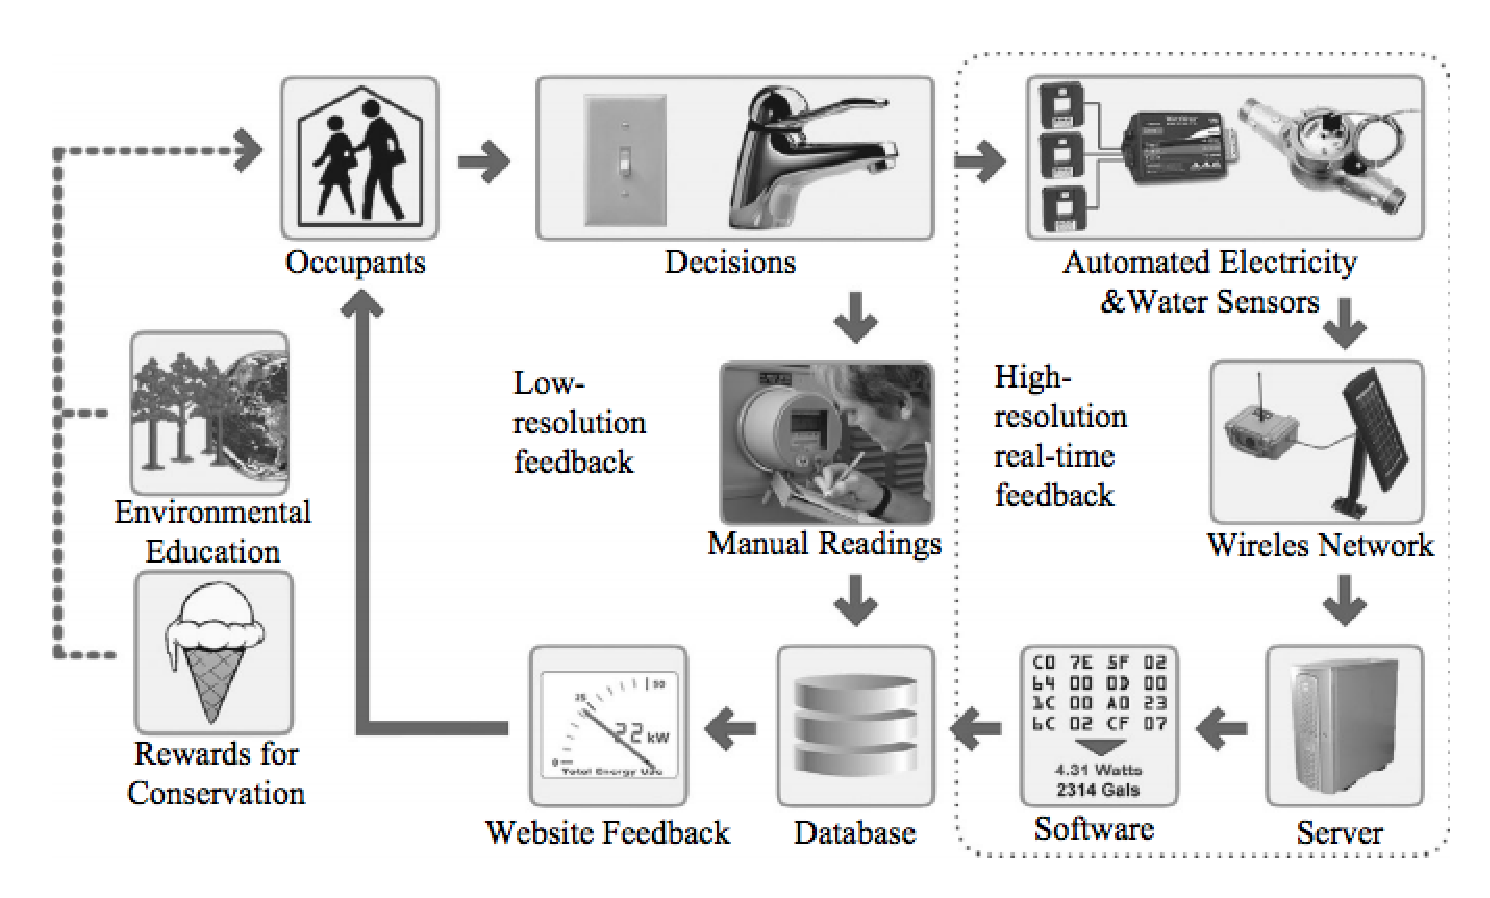
\includegraphics[width=0.6\columnwidth]{oberlin-design}
		\caption{Oberlin College's Custom Designed Sustainability Competition \cite{petersen-dorm-energy-reduction}}
		\label{fig:oberlin-design}
\end{figure}

Universities such as University of British Columbia \cite{runkle2011dark}  and Bowdoin College\cite{bowdoin} chose to out-source the technology to a commercial provider for their sustainability competition. University of British Columbia started the energy competition titled ``Do it in the Dark'' \cite{runkle2011dark} in November 2010 for the 6 first year student residence house. During the competition, the participated residence reduced overall energy consumption by 16.3\%. The competition was hosted by Lucid Design Group's Building Dashboard platform \cite{building-dashboard} which provided the online real-time feedback of energy usage for the participating residence, and other social interaction such as sharing on Facebook through the web interface. \autoref{fig:ubc-do-it-in-the-dark} shows the interface of the University of British Columbia Energy competition using the Lucid's Building Dashboard platform.

\begin{figure}[ht!]
	\centering
		
\includegraphics[width=0.6\columnwidth]{ubc-do-it-in-the-dark}
		\caption{University of British Columbia Energy Competition\cite{runkle2011dark} }
		\label{fig:ubc-do-it-in-the-dark}
\end{figure}

Campus Conservation Nationals (CCN) \cite{competetoreduce} is a nationwide electricity and water use reduction competition for colleges and universities. It has been running for the fifth year with hundreds of universities participating across North America. In 2014, 109 schools participated in the Energy Competition, which amount to total 1,330 building in the school campus and total 265,000 students and staffs actively involved in the self-chosen 3 weeks competition. Overall the competition resulted in 4.5\% average electricity competition reduction in the building level, with the top 10 schools achieved reductions ranging from 11\% to 24\%. The software infrastructure used in CCN is supported by Lucid Design Group through its the Building Dashboard platform, which is used by the participating schools to get feedback from their energy and water use, compare performance and track the competition standings.

In summary, these collegiate sustainability competitions have the same goal of engaging students in sustainability issues using resource feedback and incentives such as some kind of prizes. Some competitions also provide educational content or activities such as organizing sustainability related events. Some competitions includes a simple point scheme that participants can win points for their teams or residence dorms by participating in the events and reducing the consumption. The team or dorm with the most points will win the prize. Some competitions also include the social sharing feature such as sharing their commitments to sustainability on Facebook as a way to enforce and encourage the positive behaviors.  \autoref{table:competition} lists the comparison among these competitions. 

\begin{table}[ht!]
  \centering
        \begin{tabular}{| p{5cm} | p{1.5cm} | P{1.8cm} | c | c | p{2.5cm} |} 
        \hline
      \tabhead{School} & \tabhead{Feedback} & \tabhead{Education/ Activities} & \tabhead{Point} & \tabhead{Social} & \tabhead{Infrastructure} \\
                \hline
                Harvard University 	& manual 		& \multicolumn{1}{|c|}{\xmark}	& \xmark 		& \xmark 	& simple webpage\\
                Wellesley College  	& manual 		& \multicolumn{1}{|c|}{\xmark}	& \xmark 		& \xmark 	& simple webpage\\
                Duke University     	& manual 		& \multicolumn{1}{|c|}{\checkmark} & \checkmark & \xmark  & custom website \\
                Duke University     	& manual 		& \multicolumn{1}{|c|}{\checkmark} & \checkmark & \xmark  & custom website \\
Western Washington University & manual 		& \multicolumn{1}{|c|}{\checkmark} & \checkmark & \xmark  & custom website \\
                Oberlin College 	    	& real-time 	& \multicolumn{1}{|c|}{\checkmark} & \xmark 	& \checkmark  & custom website \\
                Bowdoin College 	& real-time 	& \multicolumn{1}{|c|}{\checkmark} & \xmark 	& \checkmark  & out-source \\
   University of British Columbia & real-time      & \multicolumn{1}{|c|}{\checkmark} & \xmark 	& \checkmark  & out-source \\
Campus Conservation Nationals  & real-time   & \multicolumn{1}{|c|}{\checkmark} & \xmark 	& \checkmark  & out-source \\
                \hline
        \end{tabular}
        \caption{University energy competitions}
        \label{table:competition}
\end{table}

None of these choices are ideal: the custom in-house solution requires sophisticated design and implementation skills; out-sourcing can be financially expensive and impedes evolution; and the simple webpage solution does not fully leverage the possibilities of advanced information technology.

The goal of Makahiki is to provide an open source framework for different organizations to create engaging sustainability serious games, including this kind of sustainability competitions. In addition to provide improvements to all of features discussed above, Makahiki creates a more game-like interface such as tracking individual points and game plays, level progression and raffle game etc. Makahiki lowers the overhead to those who would build a custom in-house solution by providing pre-built components. It can lower the financial cost to those who would out-source by providing an open source alternative. Finally, it provides an opportunity for those who would choose a minimal tech solution to instead provide more sophisticated information technology.

\section {Serious Games and Gamification}
\label{sec:rel-seriousgame}

Differentiating Makahiki from the other collegiate sustainability competition is the game design elements in Makahiki. We consider the sustainability competitions that created by the Makahiki framework are of a type of serious games.  A serious game is ``a game designed for a primary purpose other than pure entertainment'' \cite {WikipediaSeriousGame}. It includes categories such as educational games and advergames (advertising), political games, and training games (also known as game-learning). Zyda \cite{Zyda2005} defines serious game as ``a mental contest, played with a computer in accordance with specific rules that uses entertainment to further government or corporate training, education, health, etc''. 

One prominent example is Foldit \cite {khatib2011crystal}, a multiplayer online game which helps solving problems that computers can not solve very well. In this case, online gamers around the world together were able to do what biochemists have been trying to do for a decade: decipher the structure of a protein that is key to the way HIV multiplies. \autoref{fig:foldit} shows a screen shot of the Foldit game.

\begin{figure}[ht!]
	\centering
		\includegraphics[width=0.6\columnwidth]{foldit.eps}
		\caption{Serious Game Example: Foldit is solving a serious problem \cite {khatib2011crystal}} 
		\label{fig:foldit}
\end{figure}

An Alternative Reality Game (ARG) is one type of serious game related to Makahiki in the way that they both  blend real and virtual world activities in the serious gaming context. McGonigal defines ARG as ``games you play to get more out of your real life, as opposed to games you play to escape it'' \cite{mcgonigal2011reality}. Her award winning serious ARG game ``World Without Oil'' \cite{worldwithoutoil} and ``Evoke'' \cite{urgentevoke} are designed with the goal of empowering people to come up with creative solutions to urgent real-world problems. \autoref{fig:worldwithoutoil} shows an screen shot of the World Without Oil game. The game started on April 2007 for 32 days and concluded on June 2007. Approximately 2000 players participated in the game. They were asked to imagine what life would be like without oil, or try actually living without oil, then post their stories and thoughts in the forms of letter, emails, voicemails, blog posts, online videos and images. Some players reported that the online game affected their real world behaviors in some ways\cite{mcgonigal2011reality}.

\begin{figure}[ht!]
	\centering
		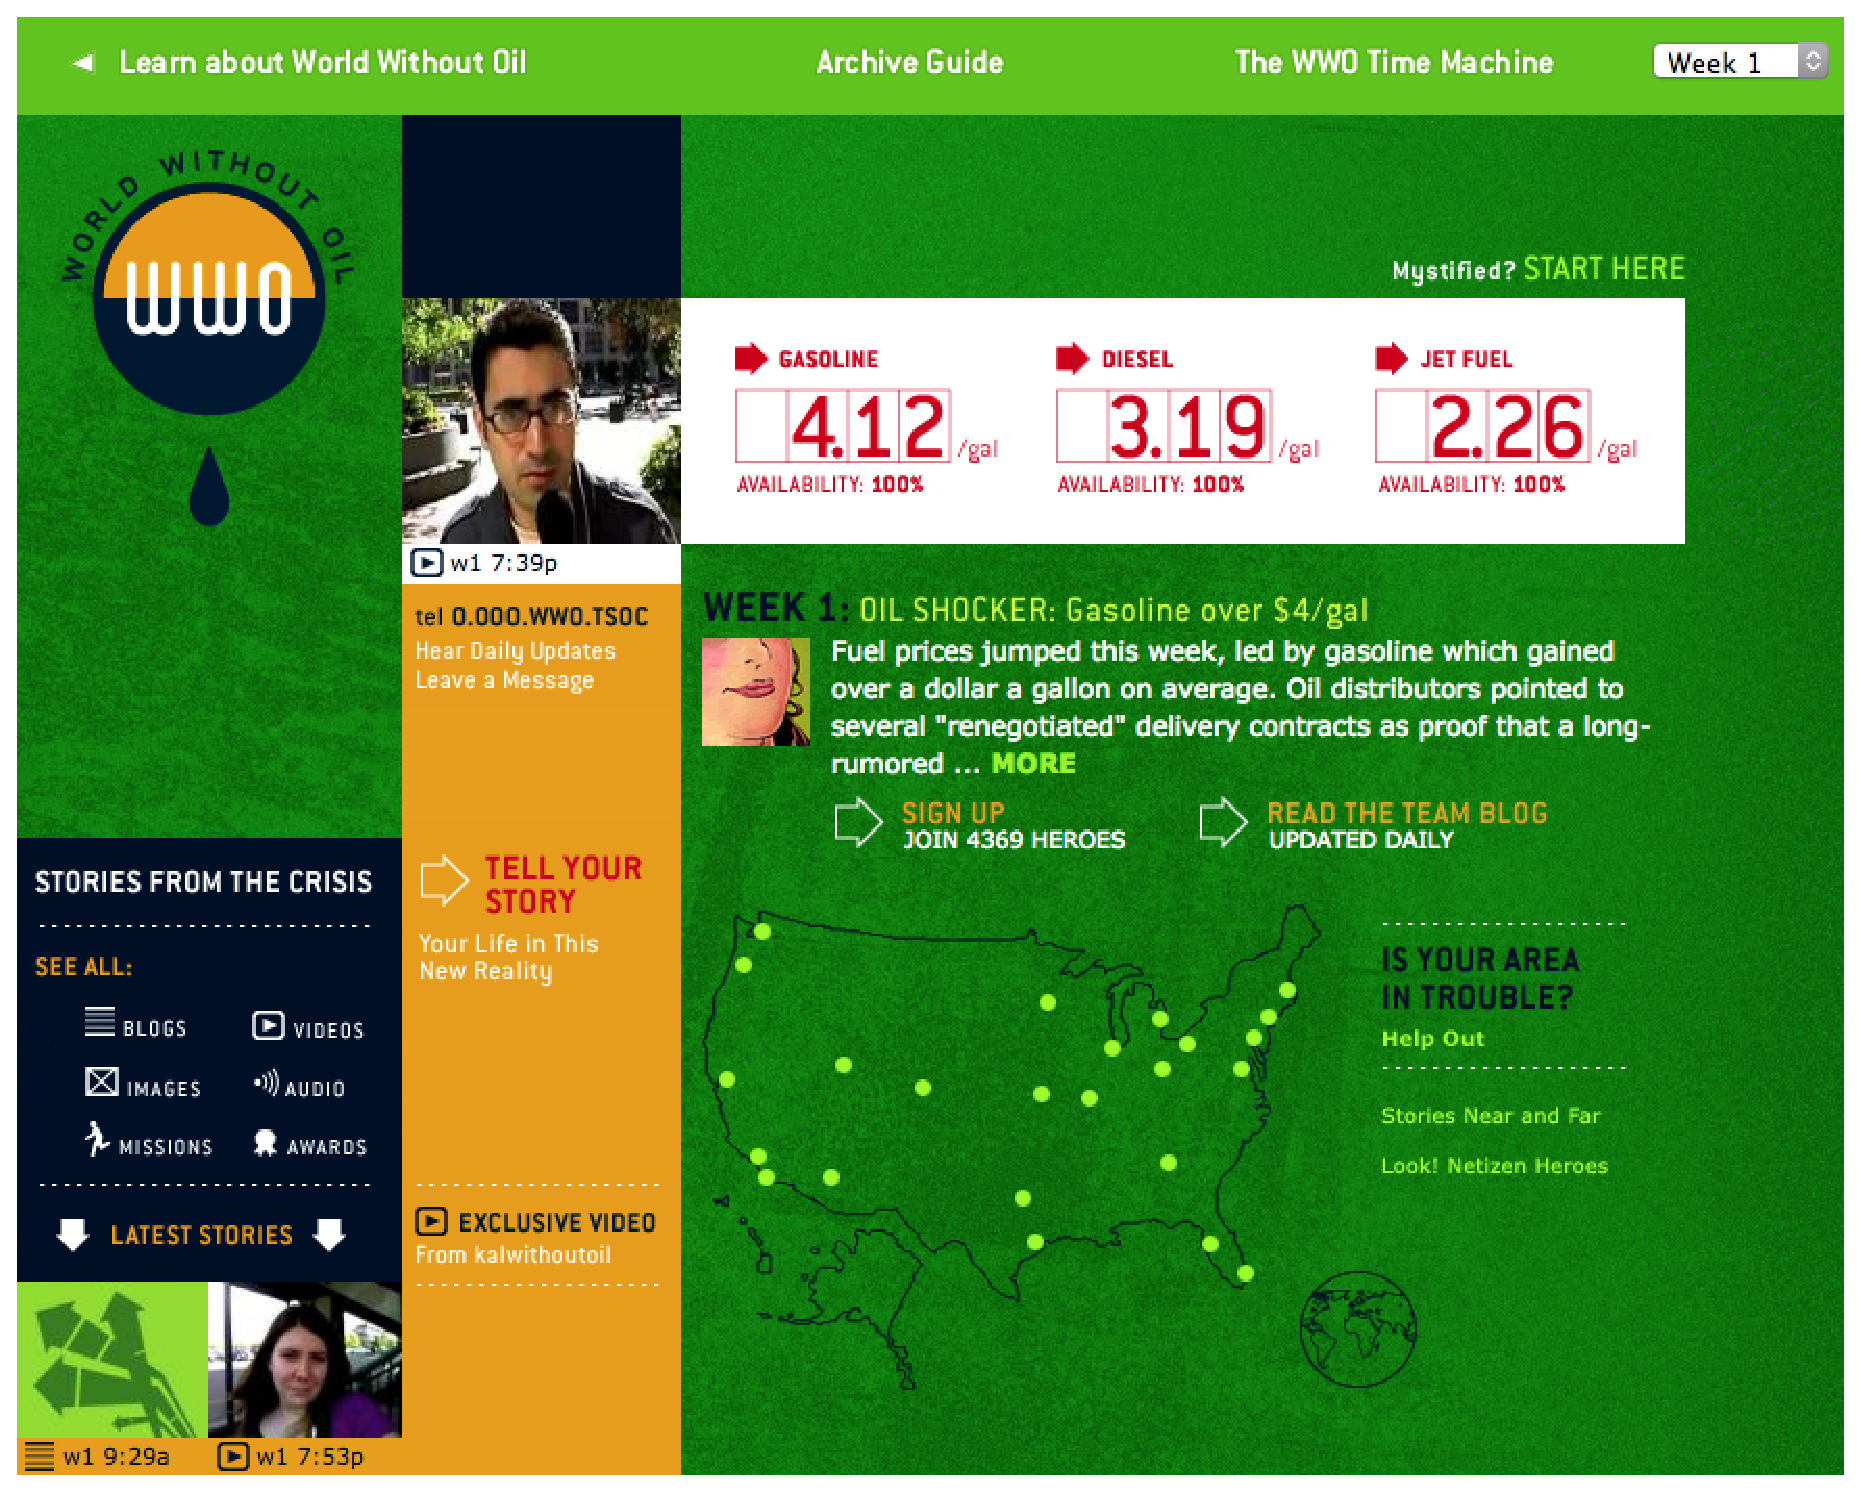
\includegraphics[width=0.6\columnwidth, height=3.5in]{worldwithoutoil}
		\caption{Serious Game Example: World Without Oil - Play it before you live it. \cite{worldwithoutoil}}
		\label{fig:worldwithoutoil}
\end{figure}

ARGs have also been used to support learning. Connolly et al. \cite{connolly2009arguing} discuss the development of an educational ARG to motivate secondary school students across Europe to learn foreign languages. The results of the pilot run of the game in 2009 indicated that 92\% of students felt the game motivated them to learn a second language. One of problems the team identified is the limitation of Moodle \cite{moodle} platform the game is based on and there is potential to improve the effectiveness of the game.

The report of the ARGOSI project \cite{whitton2009alternate} provides insights into the use of ARGs in game based learning and the challenges they face in the field of higher education. The pilot was run at the University of Bolton with the aim of providing an engaging alternative to traditional methods of introducing students to university life. Adoption of the game was fairly low with 173 players and 23 (13\%) of whom were active. The project identifies a number of questions surrounding educational ARGs, such as motivation, relationship to curriculum, marketing and timing. The report suggests that a complete ARG model may not be appropriate for wholesale learning, but there is certainly potential in using game elements.

Makahiki shares similarity with the ARGs that they both combined real and virtual world activities to achieve ``serious'' purposes, be it educational or behavior changing. 

While ``Serious Games'' has been an active research topic for decades, ``Gamification'', on the other hand, is a relatively new subject. Deterding et al. \cite {Deterding2011mt} defines gamification as ``the use of game design elements in non-game contexts''. The term only came into widespread use starting in 2010 \cite {schell2010design} \cite {zichermann2010game}. Gartner \cite {gartnerPress2011} predicts that by 2015, more than half of companies managing innovation processes will employ gamification, applying game mechanics to application areas including productivity, finance, health, sustainability, news, user-generated content and e-learning. 

Deterding et al. \cite{Deterding2011mt} describes the distinctions between gamification, serious games and other related concepts, as shown in \autoref{fig:define_gamification}. According to Deterding, a) Gamification is about games. It is different than playful interaction or playful design. b) Gamification uses game elements. It is not a complete game such as a serious game. c) Gamification applies to non-game contexts. Similar to serious games, gamification uses games for other purposes than its normal expected use for entertainment. d) Gamification focuses on design. It is not game-based technology or practice of wider game ecology.

\begin{figure}[ht!]
	\centering
		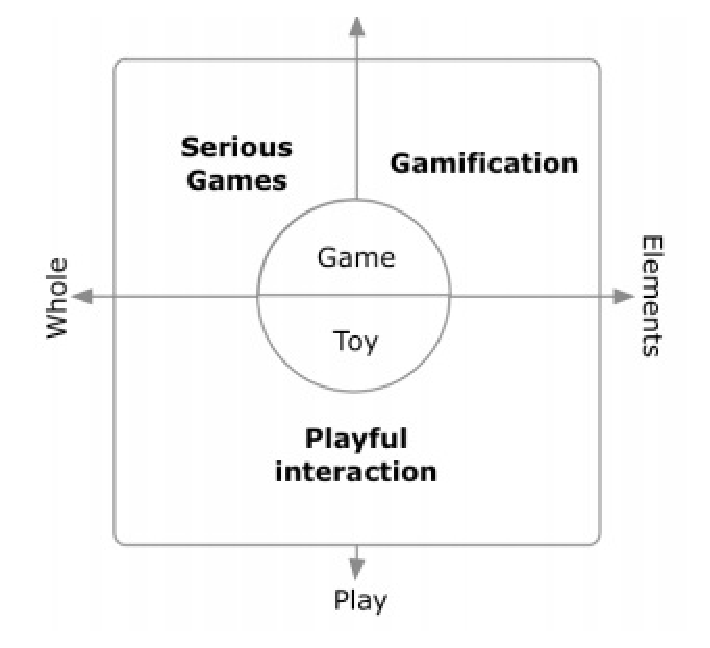
\includegraphics[width=0.5\columnwidth]{defining_gamification.eps}
		\caption{Serious Game and Gamification (source: Deterding \cite{Deterding2011mt})}
		\label{fig:define_gamification}
\end{figure}

The system created by Makahiki consists of a number of smaller games which combined,  provides a game playing experience to the participants. So we consider that Makahiki framework produces a serious game, instead of a gamified educational application. While they are different, both gamification and serious games are trying to solve problems with game thinking. Gamification's main driving force is motivation, similarly, serious games also try to solve the motivation problem and influence people's behavior for ``serious'' purpose.  Bosch \cite{bosch2011} considered the serious game Foldit as a successful example of gamification in science. 

FourSquare \cite{foursquare} is probably the most recognized example of applying game mechanics to a location based networking application. It is a location based game like service where players check-in to locations for virtual points and rewards.  By employing gamification elements such as points, badges, levels and leader boards, it engages users to revisit a location such as a restaurant or pub and become a loyal customer and finally the ``mayor'' of the place. Certain virtual rewards such as the ``mayor'' of a particular Starbucks can be converted into real products, e.g. a free coffee. Foursqure proved that simple game mechanics can affect user behavior by engaging 10 million customers with a successful business model. \autoref{fig:foursquare} shows the home page for FourSquare.

\begin{figure}[ht!]
	\centering
		\includegraphics[width=0.7\columnwidth]{foursquare.eps}
		\caption{Gamification Example: Foursquare makes modern badges popular\cite{foursquare}}
		\label{fig:foursquare}
\end{figure}

Nike+ \cite{nikeplus} is a social running game that employs game mechanics to encourage runners - both casual and hardcore - to compete and improve their fitness, with the goal of solving the main problem of most fitness programs: motivation. Nike+ allows runners to upload their exercise data to its web site, and start challenging themselves and their friends. They can also get support from their friends through the web site. The game makes running and exercise fun, which eventually serve the ``serious'' purpose of making people healthy. \autoref{fig:foursquare} shows the home page for Nike+.

\begin{figure}[ht!]
	\centering
		\includegraphics[width=0.7\columnwidth,height=3in]{nikeplus.eps}
		\caption{Gamification Example: Nike+ makes fitness run\cite{nikeplus}}
		\label{fig:nikeplus}
\end{figure}

RibbonHero \cite{ribbonhero} is a game that helps users discover new Microsoft Office features, as shown in \autoref{fig:ribbon}. The goal is to have users build familiarity and expose them to the Office UI, so that they understand what kind of features are available. According to the creator of the game, Office ``has a lot of powerful features that users might not know but can be really useful''. The game gives users a chance to learn those features through a game interface, rather than reading the software manuals or watching the typically dry IT training videos.

\begin{figure}[ht!]
	\centering
		\subfigure[Quest to earn points]{\label{fig:Ribbon1}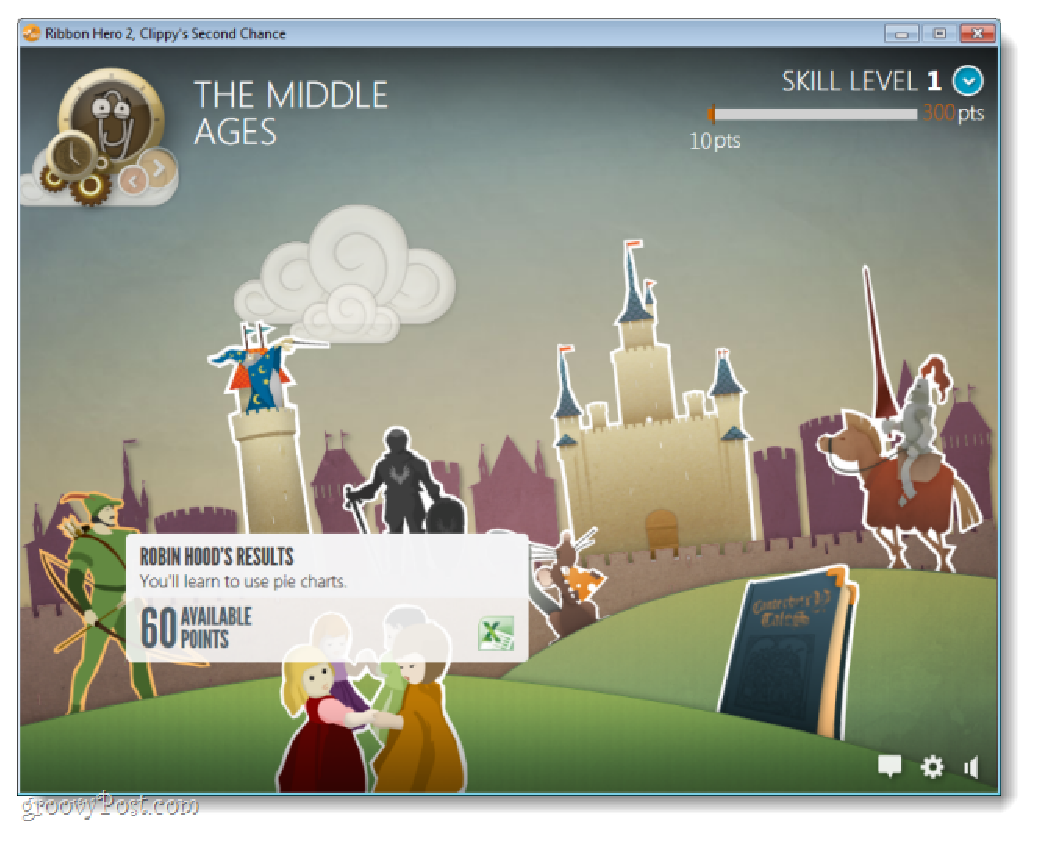
\includegraphics[height=2.5in]{ribbon1.eps}}
		\subfigure[Competing a task]{\label{fig:Ribbon2}
\includegraphics[height=2.5in]{ribbon2.eps}}
		\caption{Gamification Example: RibbonHero Helps to Learn Office\cite{ribbonhero}}
		\label{fig:ribbon}
\end{figure}

Persuasive game is another genre of video game that use game design to influence player behaviors. In his book ``Persuasive Games, The Expressive Power of Video games'', Ian Bogost\cite{bogost2007persuasive} argues that persuasive games have a unique persuasive power that goes beyond other forms of computational persuasion. Not only can
persuasive games support existing social and cultural positions, as in serious games, but they can also
disrupt and change those positions, leading to potentially significant long-term social change. Persuasive game is closely tied to ``Persuasive Technology''\cite{fogg_2003}, designed to change attitudes or behaviors of the users through persuasion and social influence, but not through coercion. Loren Baxter\cite{baxter_2011} posted that persuasive design, the use of psychology in design to influence behavior, could benefit UX design in a new level.

Interactive design also applies game elements in their design to achieve sustainability goal. One example is the ``SmartGauge'' dashboard (\autoref{fig:ixd-dashbard}) \cite {ideo2009} for Ford's hybrid cars, where a digital plant responds to how energy-efficient the users driving behavior is. The design gives drivers a game, with the goal to grow more lush and beautiful leaves, a visual reward, by driving efficiently and thus promotes a more environmental behavior. Similarly, The design of ``Piano Staircase'' (\autoref{fig:ixd-pianostair}) \cite {funtheory2009}, created by Volkswagen Sweden, installed in a metro station in Stockholm, is to make the staircase next to the escalator look and respond like a piano keyboard, so that every step on the stair will generate different piano sounds every time a commuter walked on it. Observation indicates that 66 percent more people chose to play the ``piano staircase'' game over using the escalator. It is a good example of gameful design for persuading and encouraging energy-efficient behavior. 

 \begin{figure}[ht!]
	\centering
		\subfigure[Efficiency Leaves]{\label{fig:ixd-dashbard}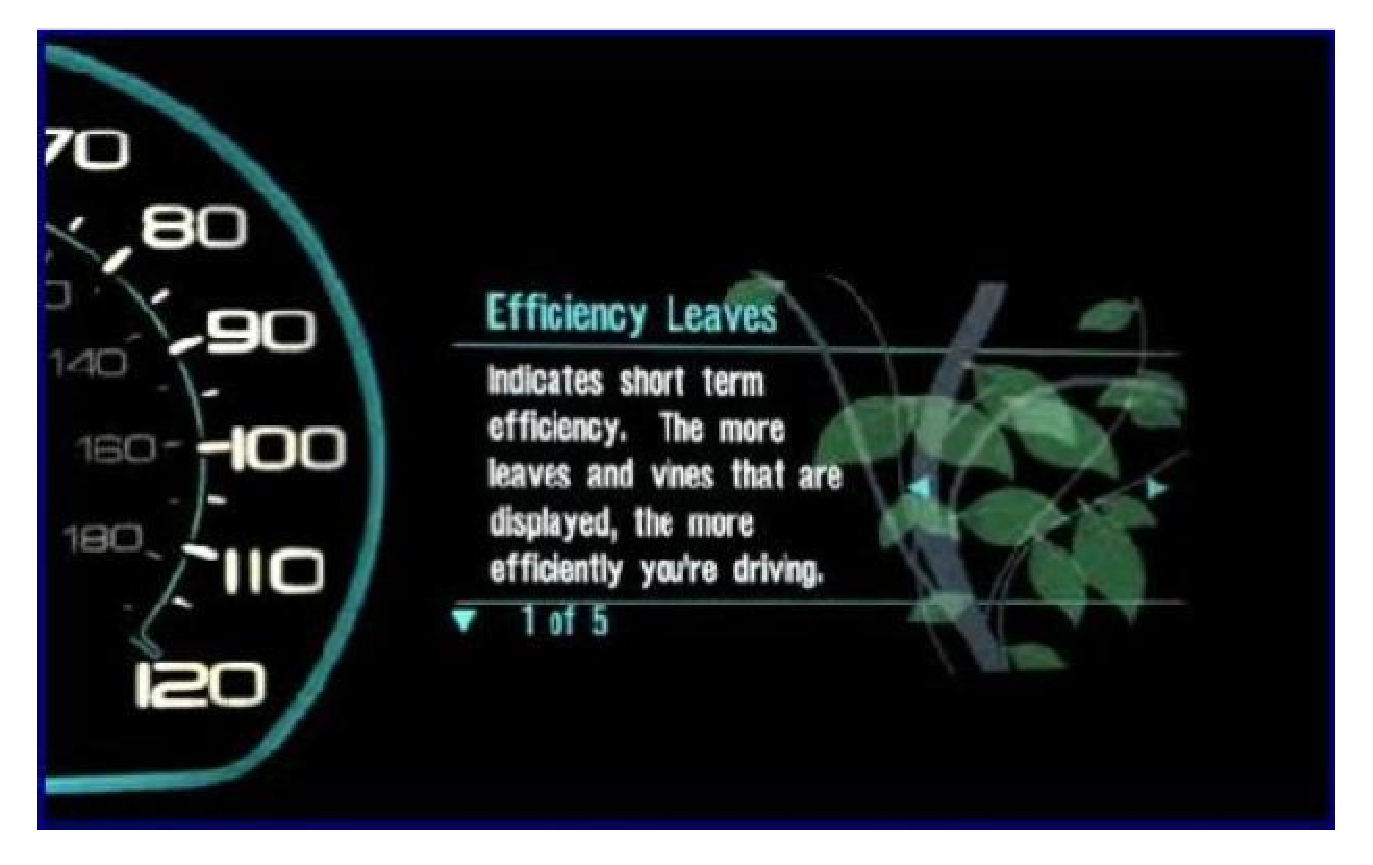
\includegraphics[width=0.6\columnwidth]{ixd-dashboard.eps}}
		\subfigure[Piano Stair vs. Escalator]{\label{fig:ixd-pianostair}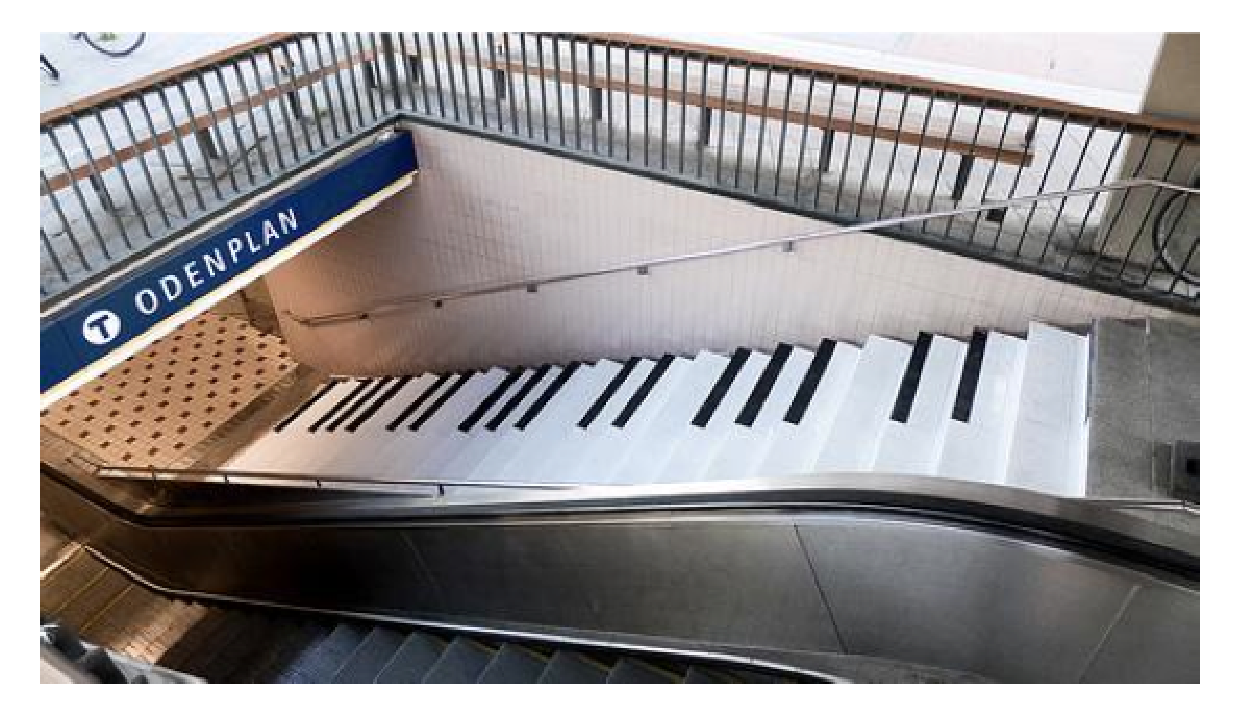
\includegraphics[width=0.6\columnwidth]{ixd-pianostair.eps}}
		\caption{Gameful Design for Sustainability}
		\label{fig:ixd}
\end{figure}	

\section{Serious Games for Sustainability}
\label{sec:rel-sg-sustainability}

Makahiki is a framework for sustainability games. Serious games for sustainability are games designed to achieve the goal of sustainability development.    

Vermontivate \cite{vermontivate}, a type of community sustainability game, shown in \autoref{fig:vermontivate}, is similar to the games created by Makahiki.  Vermontivate is a team-based game where  the players compete to accrue as many points as possible for their towns or schools by participating in a variety of sustainability-focused actions. It runs for six weeks with mainly the participants in the state of Vermont. Because of the difference between the team size, team scores are calculated ``per-capita'' by adding up a team's total points and dividing by its number of players. A new set of challenges is announced every week with a different theme such as team-building, food, energy, transportation, capital, and future action. According to the initial sponsor of the game, Vermont Energy Investment Corporation, the first Vermontivate game began in May of 2012 and attracted 225 players from 31 Vermont towns. 95\% of players reported average to above-average understanding and engagement with climate change and sustainability after playing Vermontivate, compared to 78\% prior to playing \cite{veic}. Unlike Makahiki, Vermontivate game does not have individual points or prizes and more focus on activities and relies on self-reported participation. 

\begin{figure}[ht!]
	\centering
		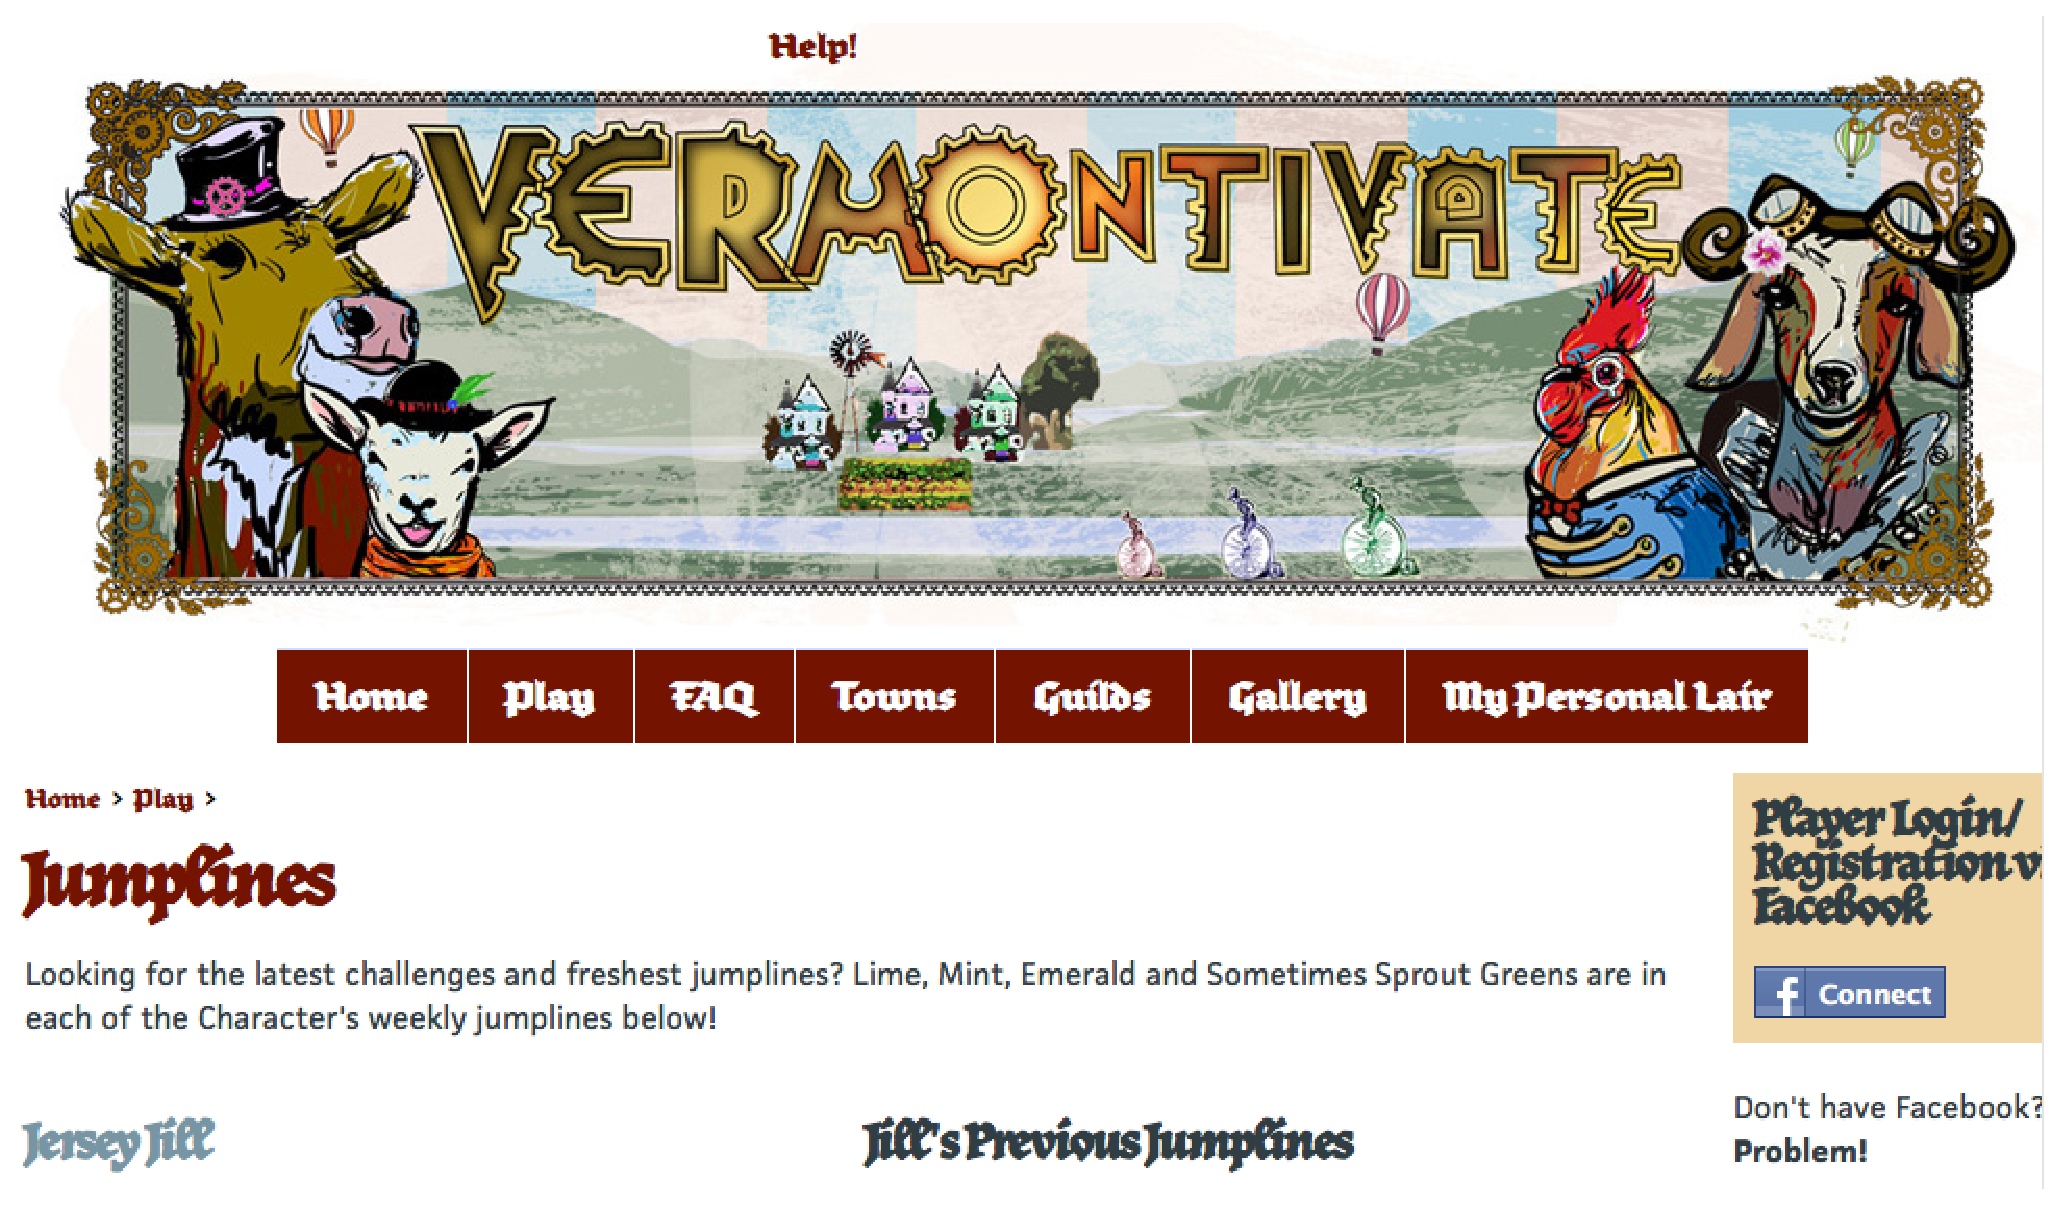
\includegraphics[width=0.6\columnwidth]{vermontivate}
		\caption{Vermontivate Sustainability Game (source: Vermontivate \cite{vermontivate})}
		\label{fig:vermontivate}
\end{figure}

Similar to Vermontivate, RecycleBank's ``Green Challenges'' \cite {recyclebank} is another serious game that used online gaming techniques to motivate participants to learn about green living and to take small green actions to live more sustainable lives offline. Figure \autoref{fig:RecycleBank1} shows a web page from the ``Green your home Challenge'' game. According to the ``Gaming For Good'' report \cite {gamingforgood}, 49,000 individuals participated in the ``Green Your Home Challenges''. Figure \autoref{fig:RecycleBank2} shows a section of the survey results regarding the self-reported sustainability behavior changes after the game. Partnered with Google Analytics and ROI research, they found that:
\begin{itemize}
	\item Gamification can increase awareness of positive environmental actions. 97\% of participants surveyed said the game increased their knowledge of the environment.
	\item Games can drive individuals to take positive social and environmental actions. Most participants surveyed indicated they are very or extremely likely to take green actions as a result of participating in the challenge.
	\item Games are an effective and appealing educational tool. 86\% participants agreed online games and contest can be a good way to inform and educate them personally.
\end{itemize}

\begin{figure}[ht!]
	\centering
		\subfigure[Green Your Home Challenge]{\label{fig:RecycleBank1}
\includegraphics[width=0.6\columnwidth]{recyclebank1.eps}}
		\subfigure[Game Change Behavior]{\label{fig:RecycleBank2}
\includegraphics[width=0.6\columnwidth]{recyclebank2.eps}}
		\caption{RecycleBank - Gaming for Good}
		\label{fig:recyclebank}
\end{figure}

The Opower Social Energy Application \cite{opower} is another kind of sustainability serious game, available as a Facebook app on both web and smartphones. It is developed in partnership with Facebook and the Natural Resources Defense Council (NRDC) with the intention of making saving energy social \cite{alliance}. \autoref{fig:opower} shows a screenshot of the game. Through the app, participants can compare their energy use to similar homes, share energy saving tips, compete with friends, and participate in team-related energy reduction challenges. The app lowers the adoption barrier by directly importing the energy usage data from Opower utility accounts. If the participant does not have an Opower utility account, he can enter data manually from his utility bills, which requires more efforts and motivation to participate. Compared to Makahiki, the energy usage feedback from Opower is not real-time (monthly), and the home energy saving tips or recommendations are not linked to points, badges, or other virtual or real rewards.

\begin{figure}[ht!]
	\centering
		
\includegraphics[width=0.6\columnwidth]{opower}
		\caption{Social Energy Application Engaging Consumers (source: Opower \cite{opower})}
		\label{fig:opower}
\end{figure}

Reeves et al. \cite{Reeves2011powerhouse} described the design of Power House, an energy game that connects home smart meters to an online multiple player game with the goal of improving home energy behavior. In the game, real world energy data is transformed into a ``more palatable and relevant form of
feedback'', and players may be incentivized by the in-game rewards to complete more energy-friendly real-world behaviors. \autoref{fig:powerhouse} shows a screenshot of the PowerHouse game. The games created by Makahiki share the similarity with PowerHouse in the way of providing real-time energy feedback to the player. Makahiki has more educational activities and less simulation game play than in PowerHouse.

\begin{figure}[ht!]
	\centering
		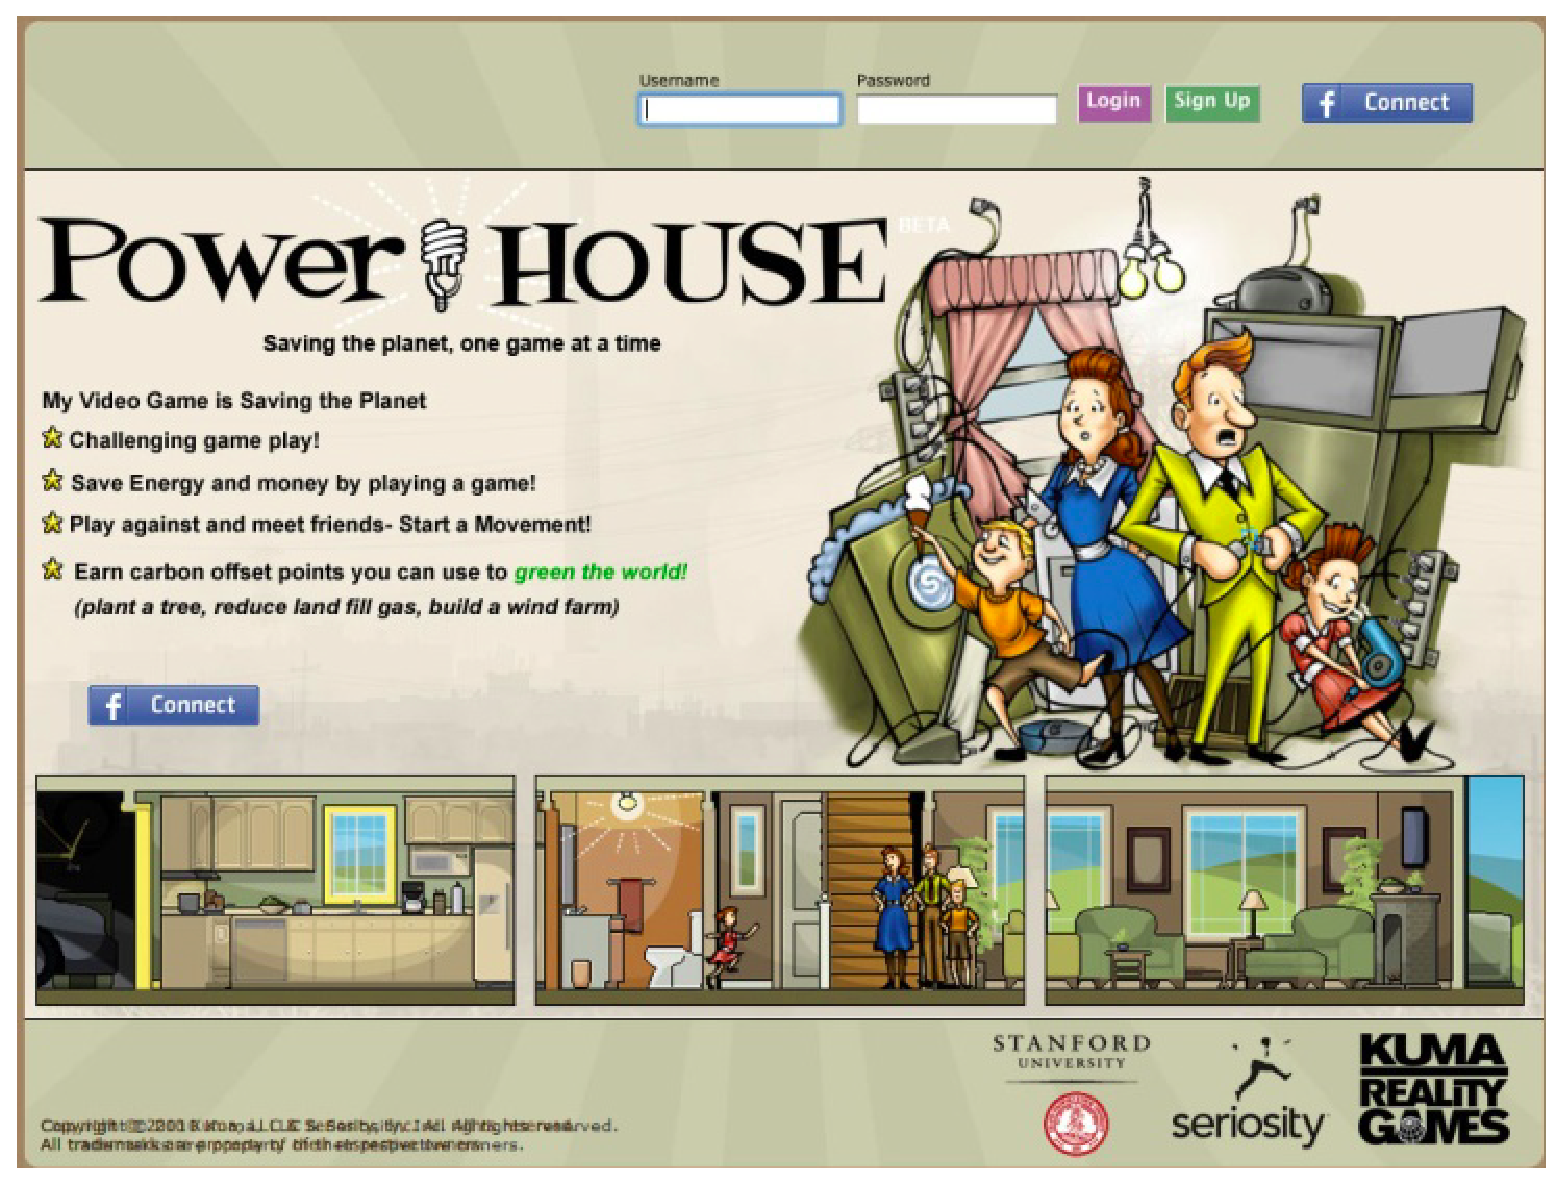
\includegraphics[width=0.6\columnwidth]{powerhouse.eps}
		\caption{Power House Game to Save Energy(source: Reeves \cite{Reeves2011powerhouse})}
		\label{fig:powerhouse}
\end{figure}

Another simulation based sustainability game worth of mention is the EnerCities \cite{enercities} developed by Dutch game developer Paladin Studios with a 1.4M budget funded by the European Commission. Awarded the title of ``Best Learning Game 2010'', offered an online learning game for young people (typical target group: 15-20 years old) to experience energy-related implications. The goal of the game is to create and expand virtual cities dealing with pollution, energy shortages, renewable energy etc. Available both as  a standalone website and on Facebook, The game was played by thousands of students from more than 110 schools across Europe. The game offers a semi-realistic simulation with cartoony 3D (via Unity3D plug-in\cite{unity3dplugin}) visual styles with multiple level game play. \autoref{fig:enercities} shows a screenshot of the game. Similar to PowerHouse game, EnerCities game engages player via the graphical simulation of the energy related issues. The player experience is more video game like than the other sustainability games such as the one's create by Makahiki. On the other hand, Makahiki as a extensible and configurable game framework, it is possible to include some simulation games such as EnerCities and PowerHouse inside Makahiki to provide better player experience and engagement.

\begin{figure}[ht!]
	\centering
		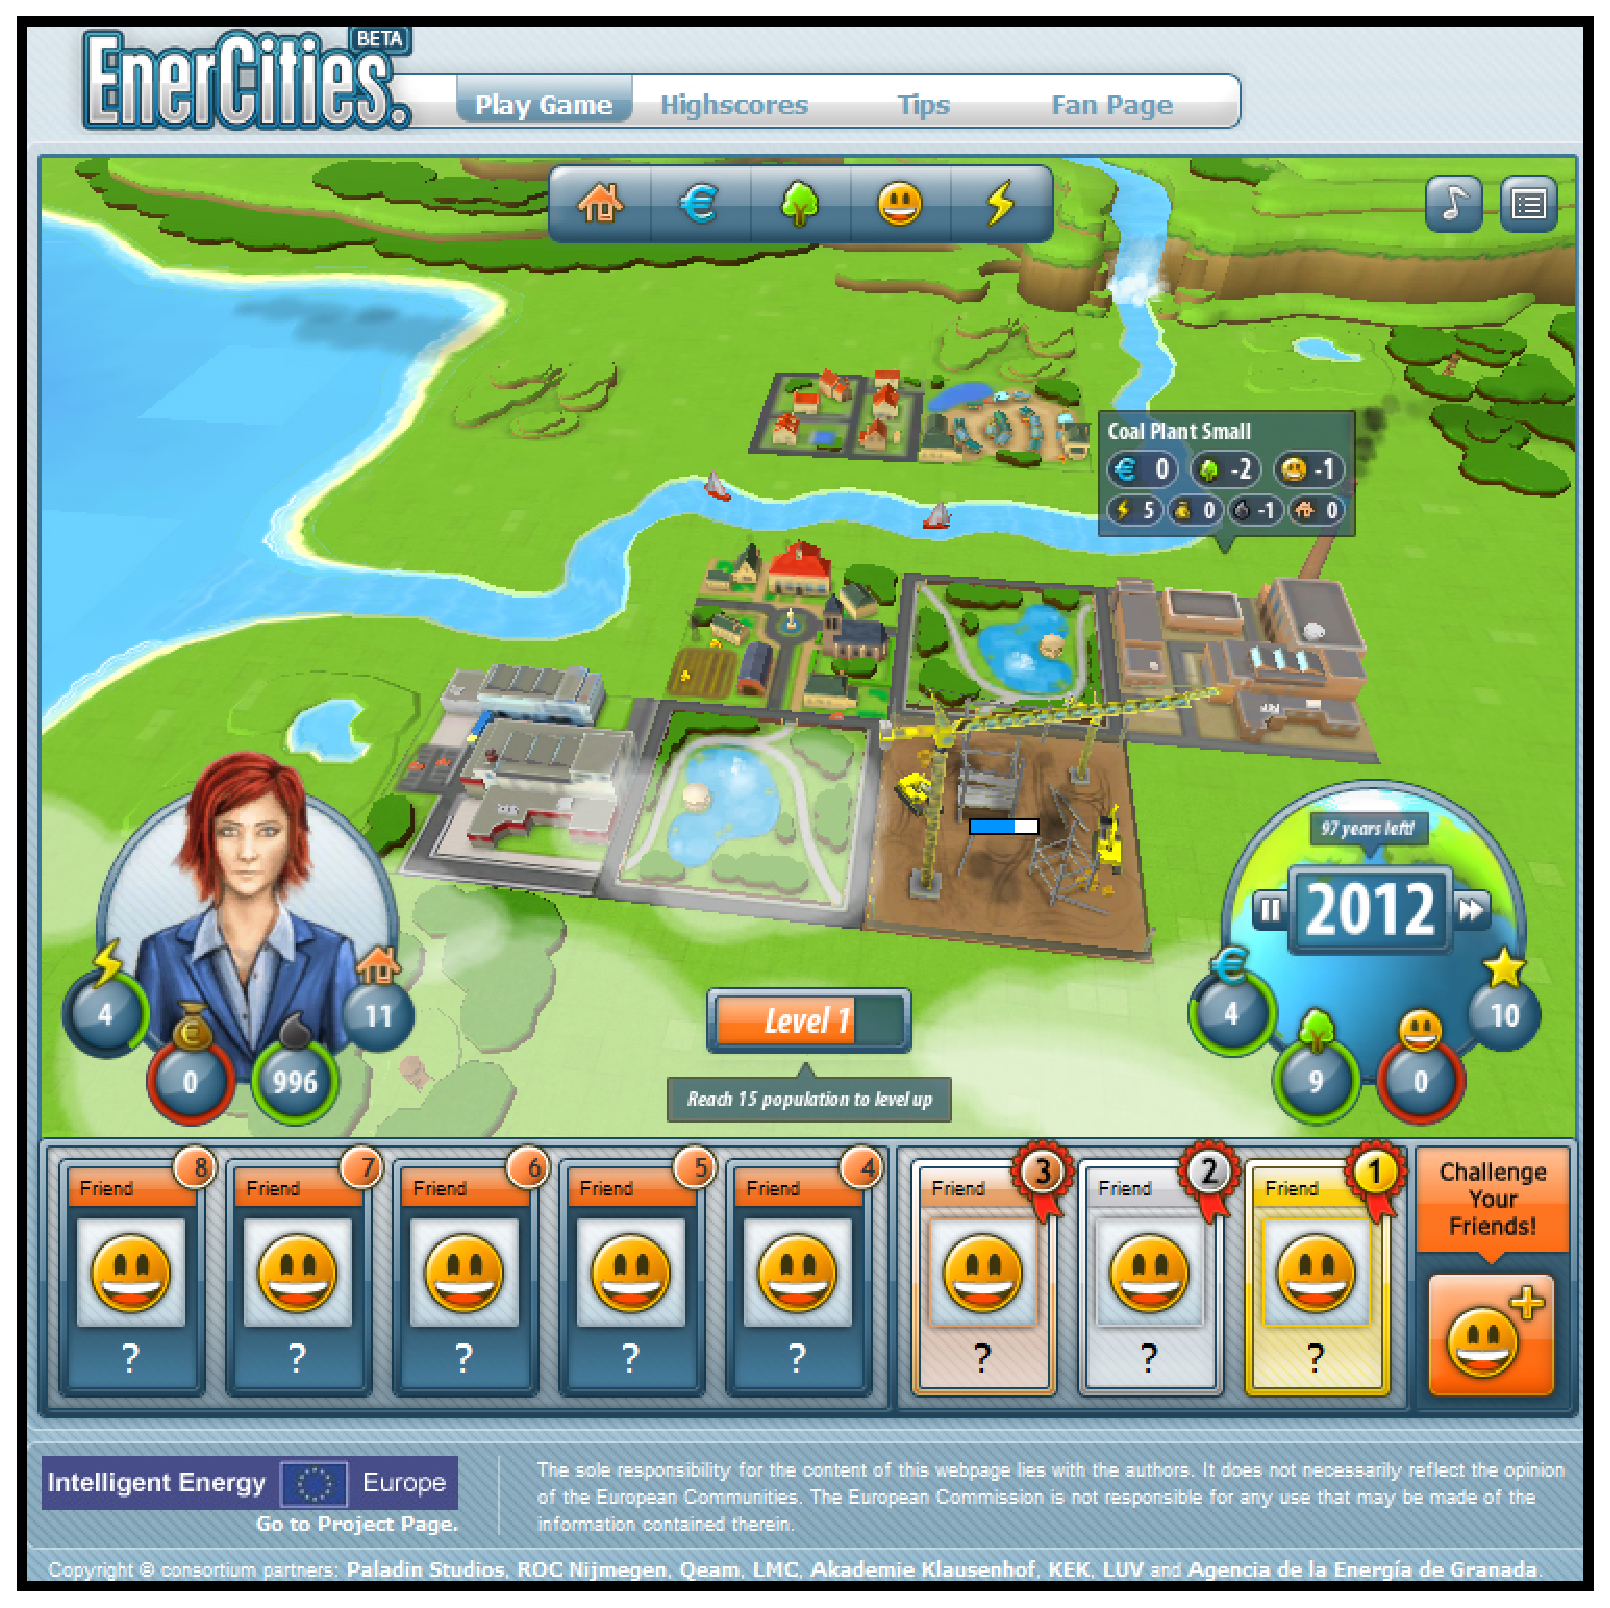
\includegraphics[width=0.6\columnwidth]{enercities}
		\caption{EnerCities - simulation based sustainability game(source: EnerCities \cite{enercities})}
		\label{fig:enercities}
\end{figure}

\autoref{table:sustainability-games} summaries the above serious games for sustainability and compares to the games created by Makahiki.

\begin{table}[ht!]
  \centering
        \begin{tabular}{| p{2.1cm} | p{2.4cm} | p{2.9cm} | P{1.5cm} | p{2cm} | c |} 
        \hline
      \tabhead{Game} & \tabhead{Type} & \tabhead{Targeted player} & \tabhead{Reward} & \tabhead{Competition} & \tabhead{Mobile} \\
        \hline
        Vermontivate 	& Website 		& Community	& Prizes & Team 	& \checkmark \\
        RecycleBank  	& Website 		& Community	& Prizes & Team	& \xmark \\
        Opower     	& Facebook App 	& Energy consumer & Virtual & Individual  & \checkmark \\
        PowerHouse     	& 2D Simulation 	& Energy consumer & Virtual & Individual  & \xmark \\
        EnerCities	    	& 3D Simulation 	& Schools & Virtual	& Individual  & \xmark \\
	Makahiki		& Website		& Schools & Prizes \& virtual & Team \& individual  & \checkmark \\
        \hline
        \end{tabular}
        \caption{Serious games for sustainability}
        \label{table:sustainability-games}
\end{table}

\section{Game Design and Motivation}
\label{sec:game-design}

The research in serious games and gamification inspires the design of Makahiki in terms of benefits of a game, game design and how the game design can motivate and engage players in serious contexts. 

Why games? Results of a study published in the May 1998 issue of Nature \cite {koepp1998evidence} demonstrated that video game players experience regular releases of dopamine during game play. Dopamine is a neurotransmitter that signals pleasure rewards for food, sex and addictive drugs, such as cocaine. 

A favorite subject of Greek vase paintings in the ancient games exhibition in the British Museum's department of Greek and Roman antiquities is Ajax and Achilles playing a kind of board game called backgammon, as illustrated in \autoref{fig:ancient-games}. It is noteworthy that both Ajax and Achilles have the full armor on while playing the game. According to Arthur A. Krentz \cite{krentz1998play}, in Plato's ``Republic'', the term ``paideia" (in Greek, means education/culture), ``paidia" (means play/game/pastime/sport), and ``paides" (means children), have the same root. The three terms often show up in the same context. Krentz states that ``The central aim of pedagogy (paidagogia) is to encourage learning as a form of play (paidia), which is the most persuasive and effective approach to learning" .

\begin{figure}[ht!]
	\centering
		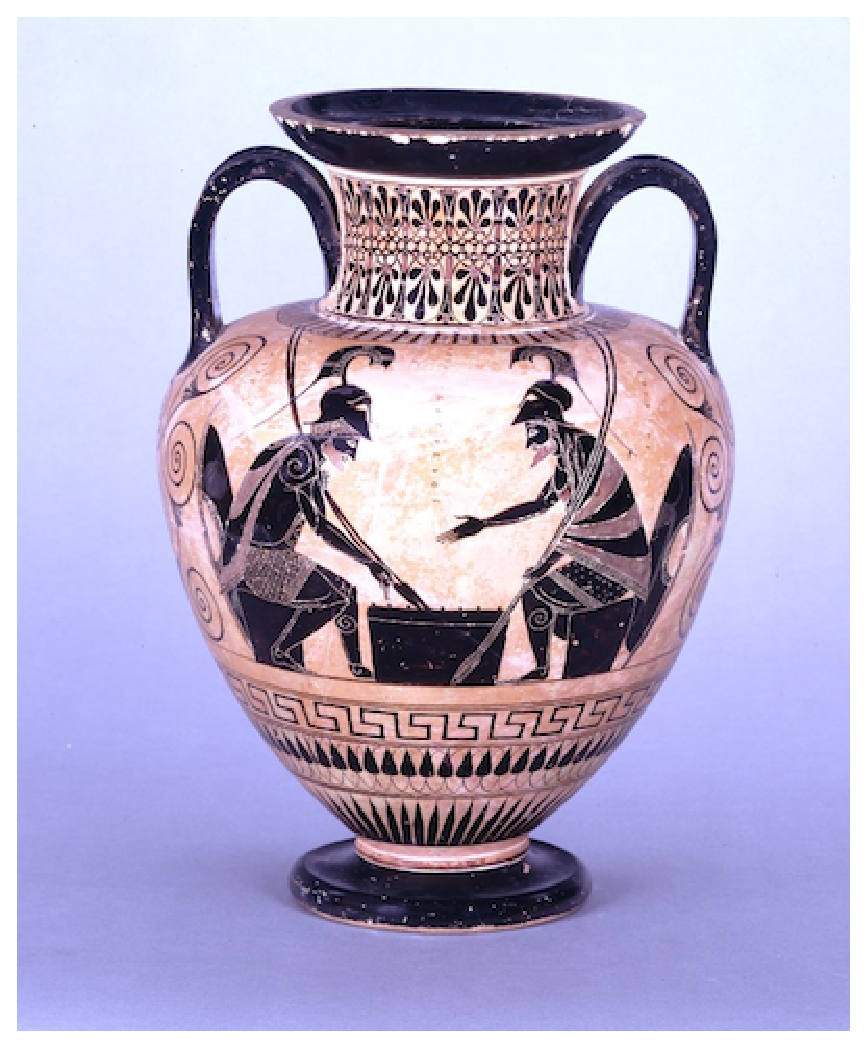
\includegraphics[width=0.4\columnwidth]{roman-game-vase.eps}
		\caption{Ancient Games Shown in British Museum}
		\label{fig:ancient-games}
\end{figure}

Moving forward a couple of millennia, World of Warcraft (WoW) is a massively multiplayer online role-playing game (MMORPG) with 11.1 million subscribers, currently the world's most popular MMORPG.  Nick Yee \cite {yee2002understanding} pointed out that the collaborative nature of most activities makes MMORPG unique. ``It's the people that are addictive, not the game''. ``Most importantly, it is the reward of being socialized into a community of gamers and acquiring a reputation within it''  . He claimed \cite {yee2001vsb} that ``WoW truly is a virtual Skinner box'', smoothly increasing reward and difficulty and reinforcing player commitment along the way.
	
In her popular and inspiring TED talk ``Gaming can make a better world" \cite {mcgonigal2010ted} and in her book ``Reality is Broken" \cite {mcgonigal2011reality}, researcher and game designer Jane McGonigal makes a case for why good games make us better, and how they can help us change the world. She notes that more than 3 billion hours a week is spent in playing video game by our society. She says that the average gamer plays 10,000 hours of games by age 21. That's about the same number of hours that students spend in high school and middle school. There are 500 million gamers today, playing on all sorts of platforms from the iPhone to game consoles. Instead of the common conception that gaming is a waste of time, she argues that ``playing games is the single most productive thing we can do with our time'' and that is  the solution to our ``Broken Reality''. Byron Reeves also argues in his book ``Total Engagement" \cite {reeves2009total}, that games, especially MMO type games, can change the way people work and businesses compete.

Psychology professor Mihaly Czikszentmihalyi introduced a specific kind of happiness that he named ``flow" \cite{csikszentmihalyi1991flow}, which is considered as one of the fundamental reasons that people play games \cite{murphygames}. Flow is a state of absorption, characterized by intense concentration, loss of self-awareness, a feeling of being perfectly challenged (neither bored nor overwhelmed) and a sense that time is flying. In order to achieve flow, the important condition is a balanced goal that is challenging yet achievable within the individual's ability. This balance is referred to as the flow channel as shown in \autoref{fig:state_of_flow}.

\begin{figure}[ht!]
	\centering
		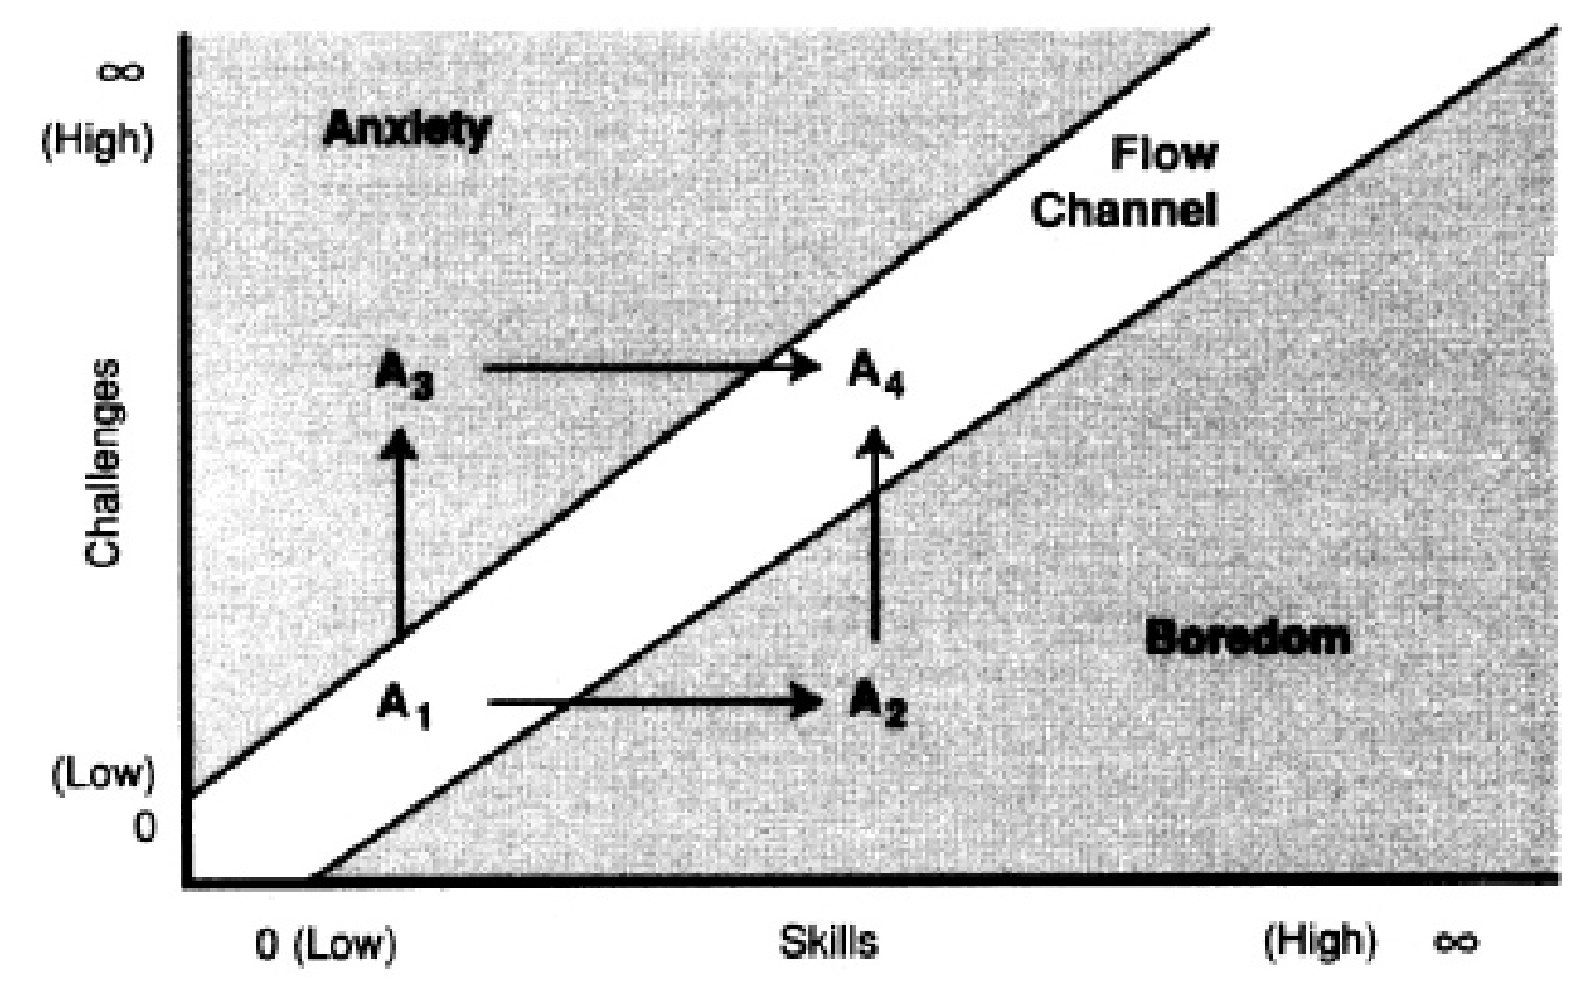
\includegraphics[width=0.7\columnwidth]{flow.eps}
		\caption{The state of flow is achieved between anxiety and boredom \cite{csikszentmihalyi1991flow}}
		\label{fig:state_of_flow}
\end{figure}

In order to understand why people play games, Richard Bartle identified four player personality types by studying players of the Multi-User Dungeon (MUD) game in 1960s \cite {bartle1996hearts}:
\begin{enumerate}

\item \textbf{Achievers}: driven by in-game goals, usually some form of points gathering - whether experience points, levels, or money.

\item \textbf{Explorers}:  driven to find out as much as they can about the virtual construct - including mapping its geography and understanding the game mechanics.

\item \textbf{Socializers}: use the virtual construct to converse and role-play with their fellow gamers.

\item \textbf{Killers}: use the virtual construct to cause distress on other players, and gain satisfaction from inflicting anxiety and pain on others.

\end{enumerate}

Bartle's player type model has been the basic for understanding the player motivation. Dan Dixon presented the limitation and misuse of Bartle's model in general games and gamification contexts \cite{DixonPlayerType}. Amy Jo Kim applied the model in her gamification approach by overlaying social actions from the game on top of the player types \cite {Kim2010}, as shown in \autoref{fig:play-types}.

\begin{figure}[ht!]
	\centering
		\subfigure[Bartle's Player Types (1996)]{\label{fig:player-types}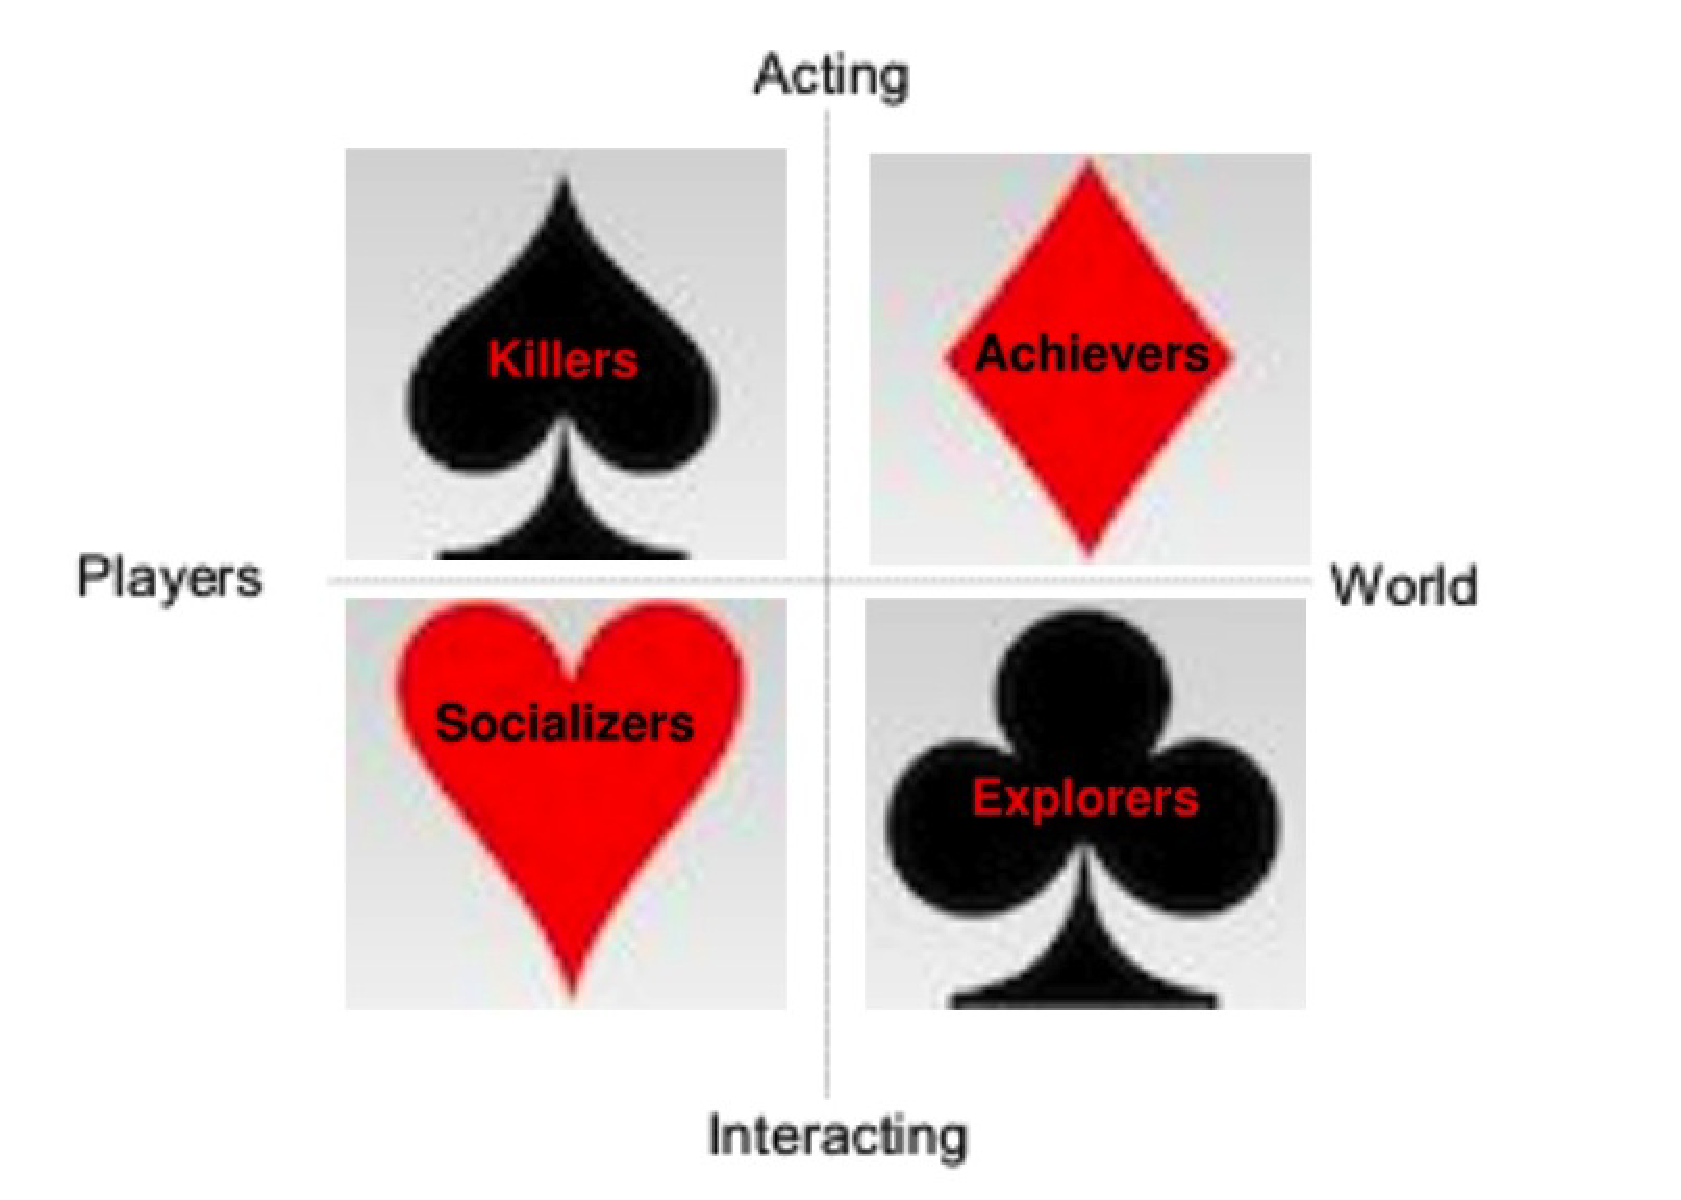
\includegraphics[height=2.1in]{bartle-player-types.eps}}
		\subfigure[Kim's Social Actions (2010)]{\label{fig:social-action}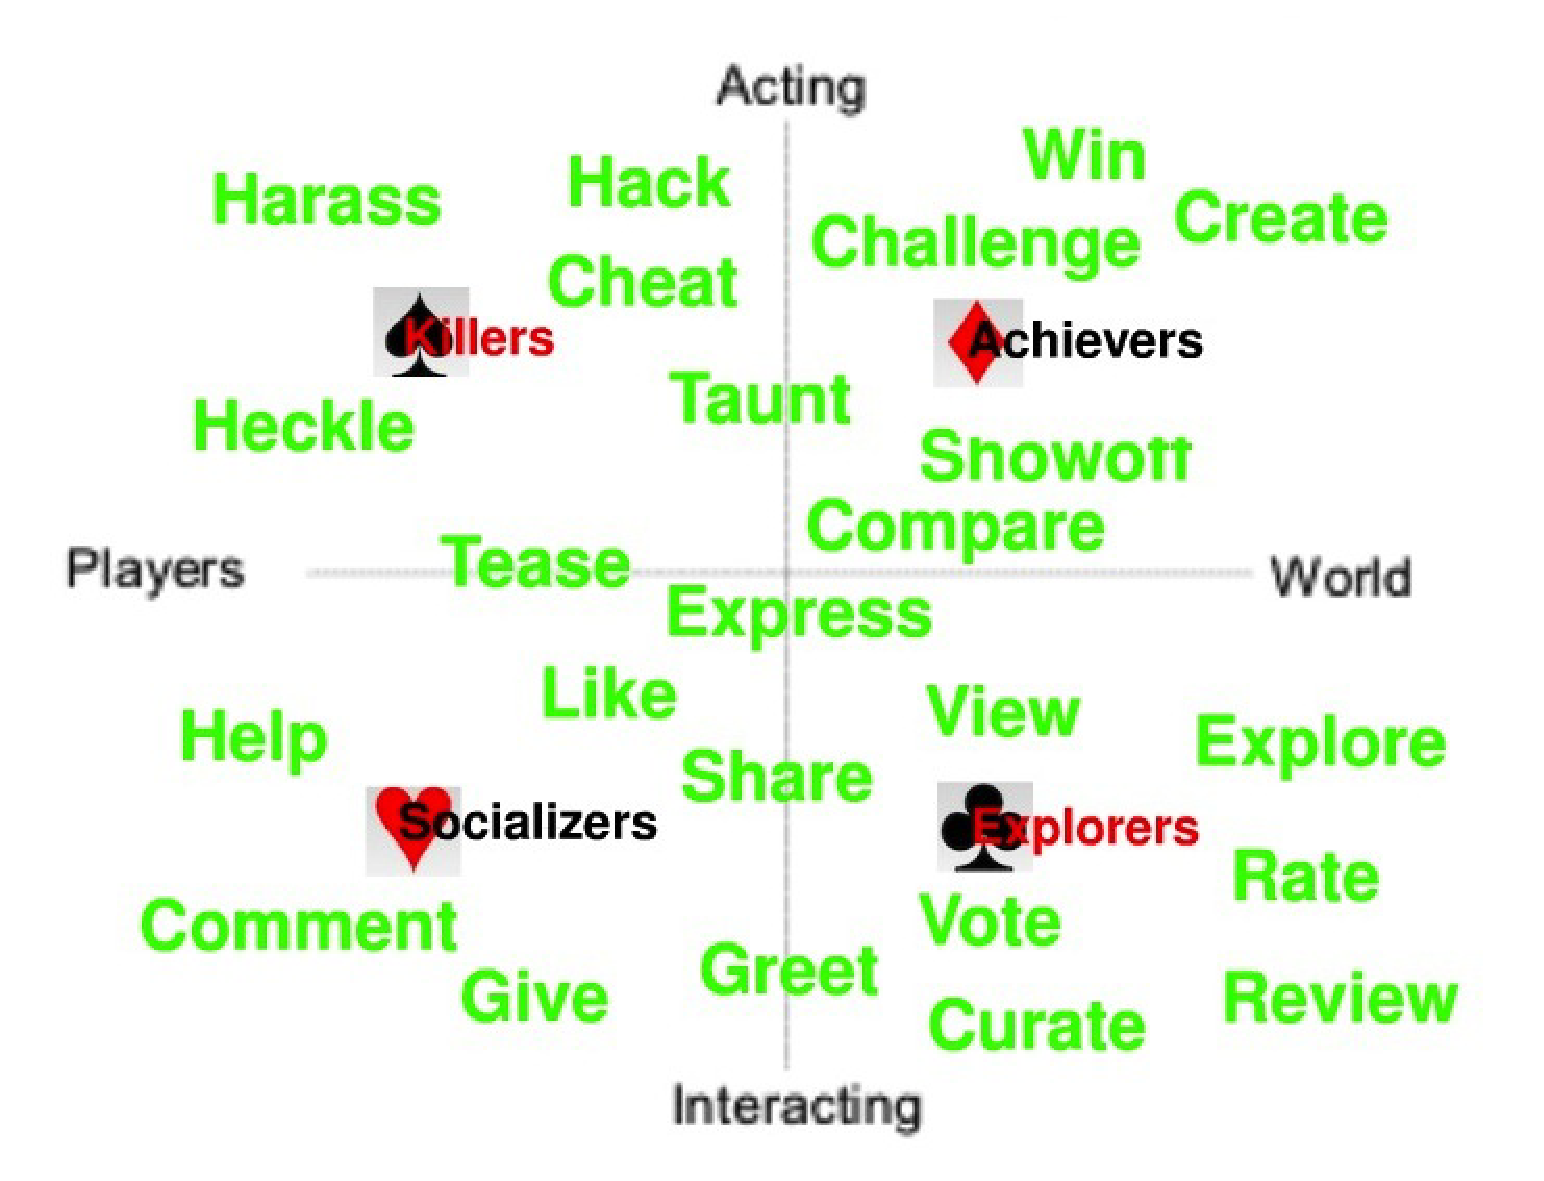
\includegraphics[height=2.1in]{kim-player-types.eps}}
		\caption{Player Types}
		\label{fig:play-types}
\end{figure}

Different game mechanics and elements can be used to serve different functions in satisfying players' needs, and the basic elements such as points, badges, and leader boards are the defining attributes of the current gamification practices \cite {Deterding2011dragon}. \autoref{fig:basic-game-elements}  illustrates these basic game mechanics and elements.

\begin{figure}[ht!]
	\centering
		\subfigure[Satisfies Human Needs (source: Bunchball\cite{bunchball})]{\label{fig:human-needs}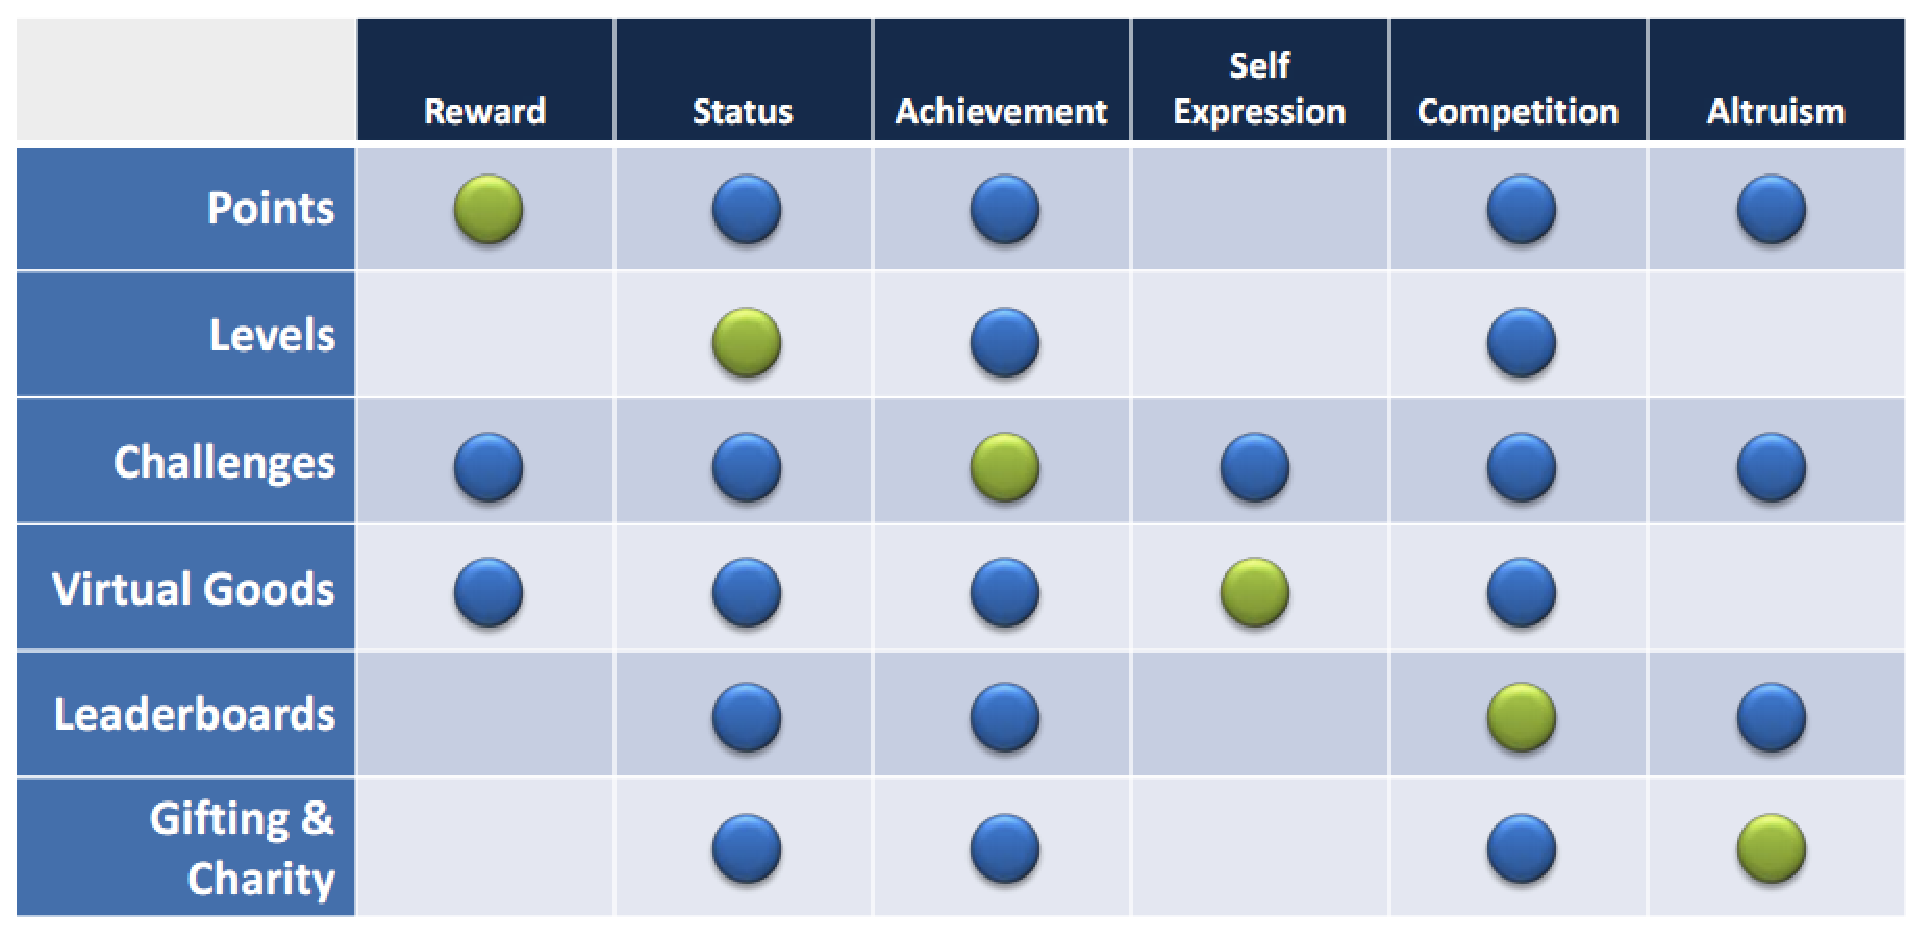
\includegraphics[width=3.8in]{human-needs.eps}}
		\subfigure[Basic Mechanics (source: Deterding \cite{Deterding2011meaningful})]{\label{fig:basic-elements (source: }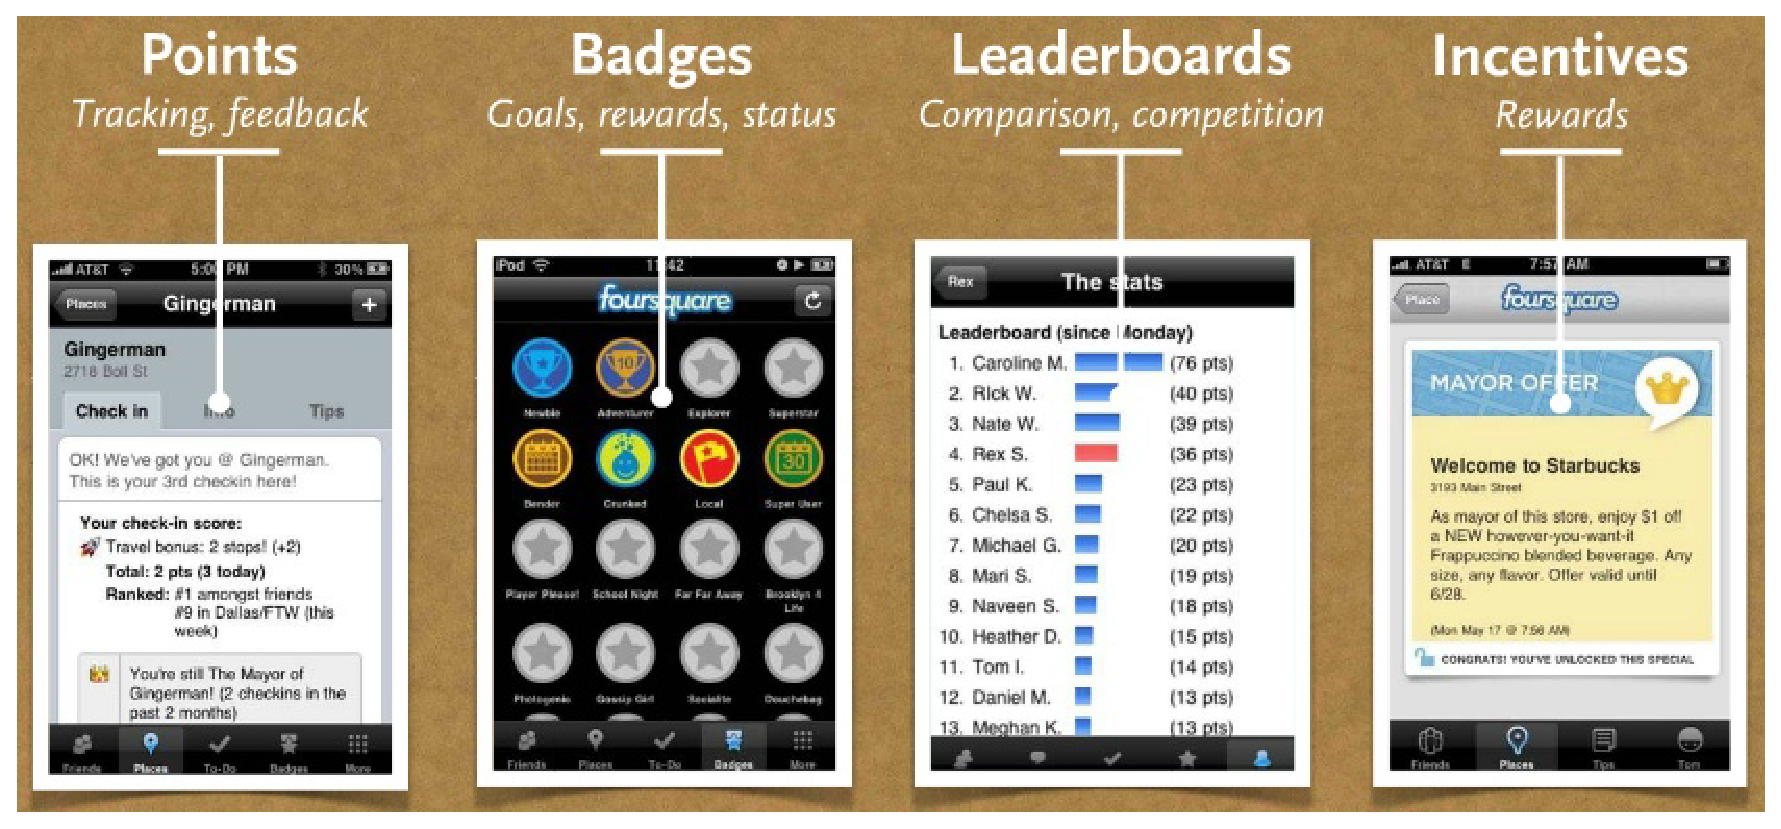
\includegraphics[width=3.8in,height=2in]{basic-element.eps}}
		\caption{Basic game mechanics and elements}
		\label{fig:basic-game-elements}
\end{figure}

Seth Priebatsch \cite {Priebatsch2010ted} stated that you can get anyone to do anything with 7 game dynamics. Techcrunch \cite{Biggs2010} published a ``secret'' game dynamics play deck that is used by Priebatsch's company SCVNGR. The play deck is a set of 47 flash cards. Each card illustrates one game dynamics. SCVNGR employees are instructed to memorize them and apply in their applications as needed.  

There are many debates and criticism over whether gamification itself is inherently good or bad. 
Many considered the current efforts of gamification focus on extrinsic motivators (such as points, badges and rewards) instead of intrinsic motivators generated by an individual's internal will or desires.

Designer Stephen Anderson claimed that gamification mistakes extrinsic rewards (rather than intrinsic motivation) for the power of games and hence offers only feedback, not goals \& rules \cite {anderson2011}. 

\begin{figure}[ht!]
	\centering
		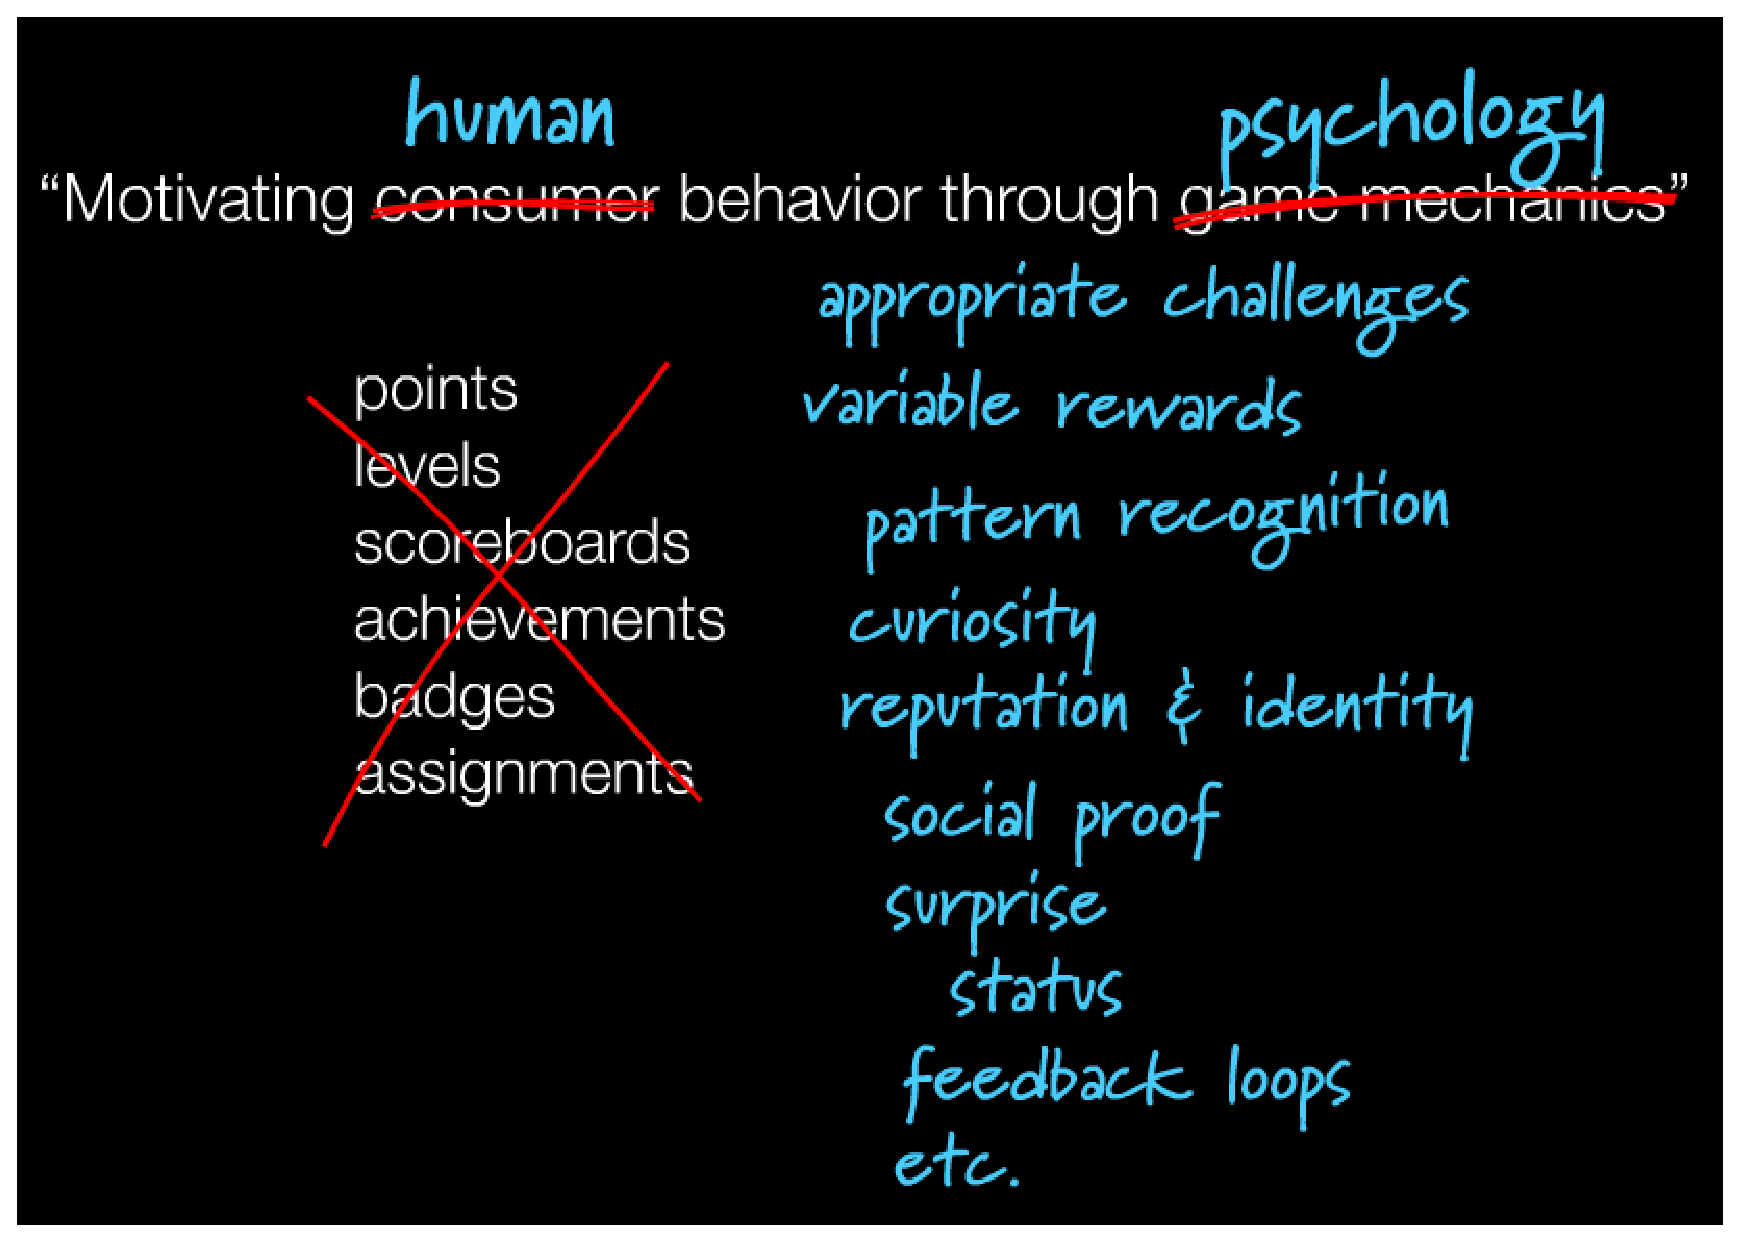
\includegraphics[width=0.6\columnwidth]{anti-gamification.eps}
		\caption{Gamification is about extrinsic rewards (source: Anderson \cite {anderson2011})}
		\label{fig:anti-gamification}
\end{figure}

Jane McGonigal spoke about her concern about current state of gamification in the GDC 2011 talk titled ``We don't need no stinking badges: How to reinvent reality without gamification'' \cite {mcgonigal2011}. She argued that current gamification confuses intrinsic/extrinsic motivation and proposed ``Gameful Design'' instead of ``Gamification''. She claimed that "Gameful is player-oriented", which presumed that the loyalty program type gamification is product or service oriented. While the current gamification is about extrinsic reward, with points, badges, and levels, gameful design is about intrinsic reward, with positive emotion, relationships, meaning and accomplishment.

Nicole Lazzaro argued that the use of extrinsic rewards will decrease the motivation to use your products and services once you remove that reward \cite {Lazzaro2011}. Vockell resonated that in education psychology, extrinsic motivators may lead to short-range activity increase but reduction in long-range interest in a topic. While intrinsic motivators motivate people best when they are working toward personally meaningful goals \cite{vockell2004educational}. 

Michael Wu argues that extrinsic rewards can jumpstart intrinsic motivation  \cite {WuSustainable2011}. He claimed that gamification just has to work long enough for some other processes to take over as the primary driver of value. Subsequently, it becomes a secondary reinforcement system. 

In order to design a game that that is intrinsic motivated, Amy Jo Kim presented ``Smart Gamification'' which focuses on designing an effective ``Player Journey'' with intrinsic reward preferred over extrinsic reward \cite {Kim2010}. Kim pointed out that intrinsic values are greater than extrinsic rewards and ``a good game take the player on a journey toward mastery". As illustrated in \autoref{fig:player-lifecycle}, when over time players progress from newcomer to regular and finally to enthusiast, they progress from novice to expert to master. Kim also incorporates the MDA framework \cite {hunicke2004mda} by using it to guide and motivate the player journey as illustrated in \autoref{fig:game-design}.

\begin{figure}[ht!]
	\centering
		\subfigure[Player Journey]{\label{fig:player-lifecycle}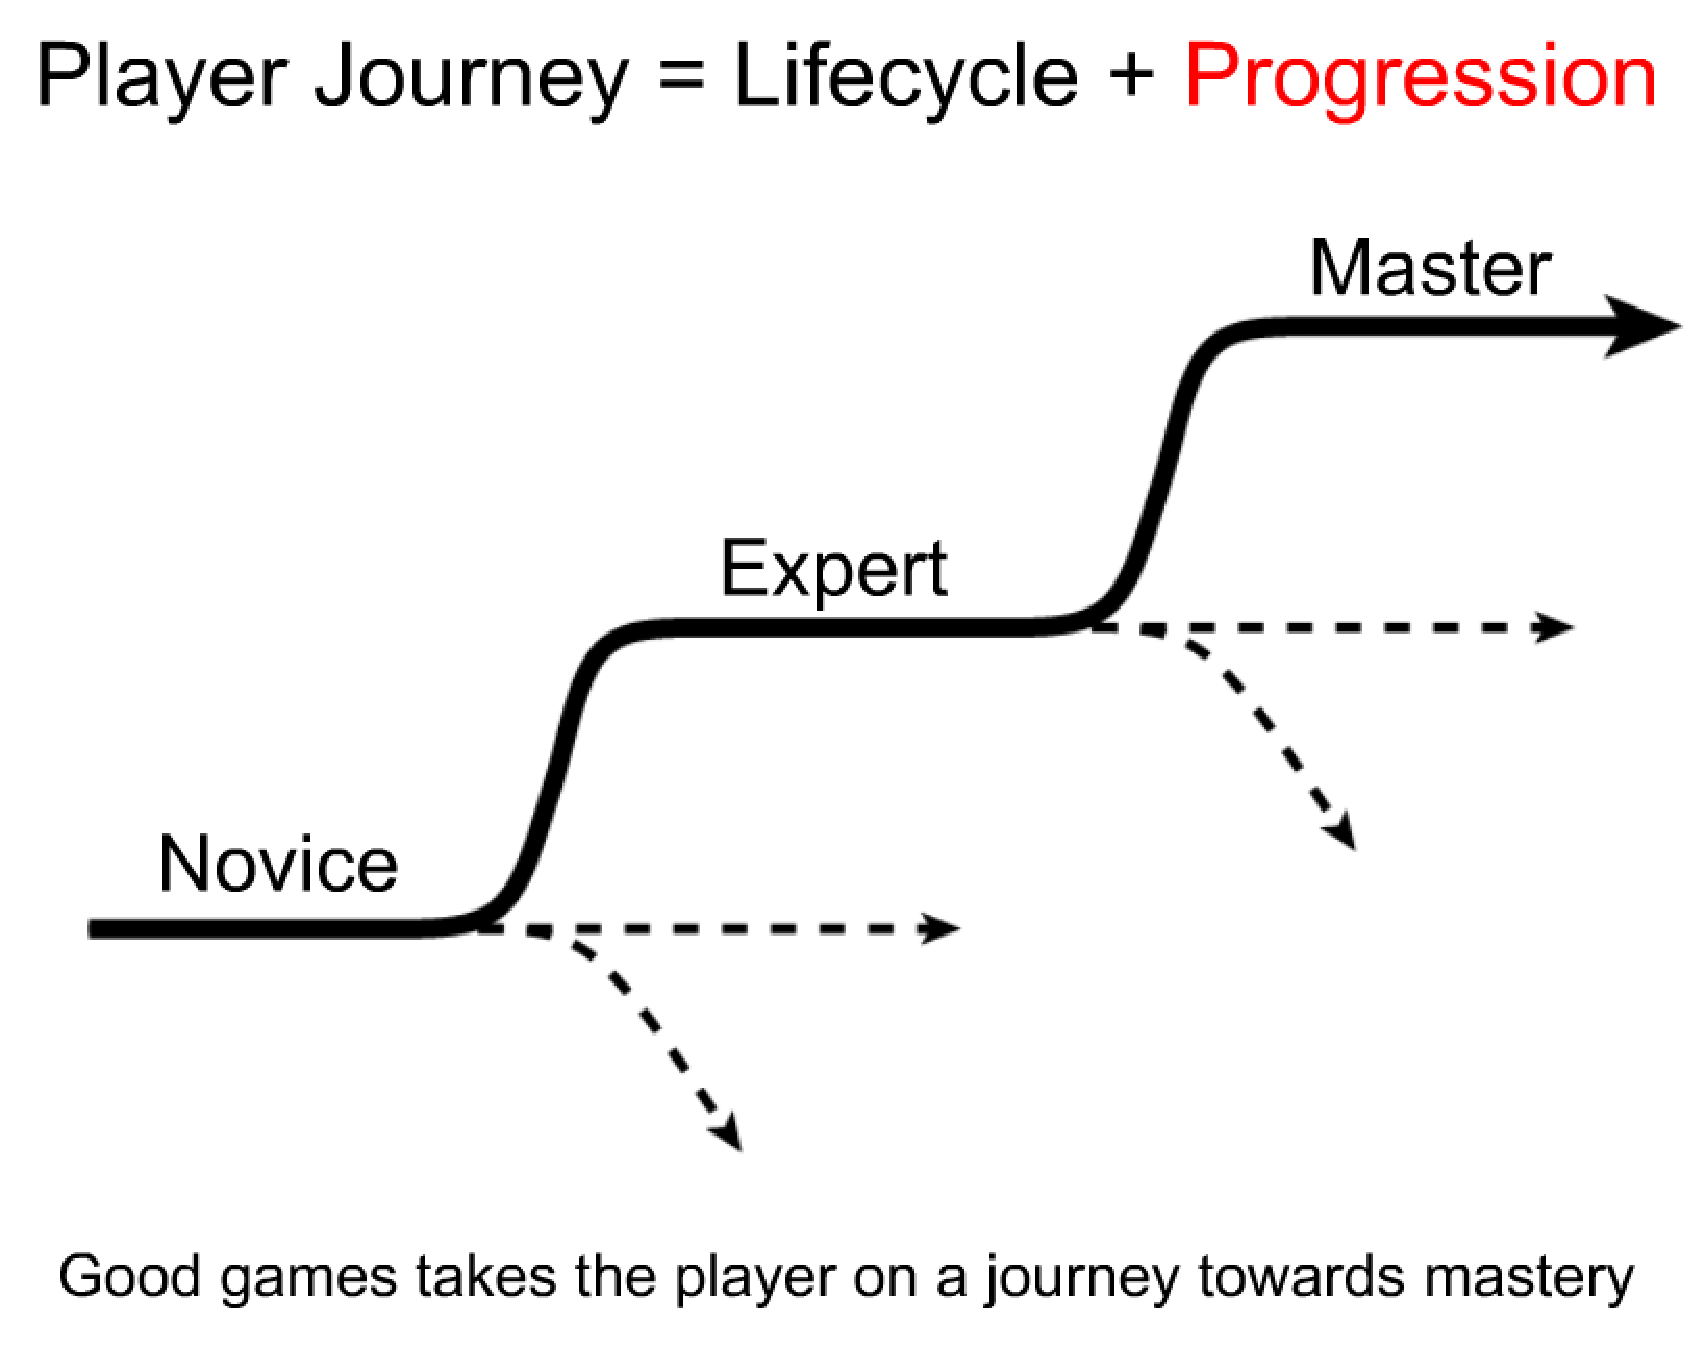
\includegraphics[height=2.1in]{kim-workshop.eps}}
		\subfigure[Game Design]{\label{fig:game-design}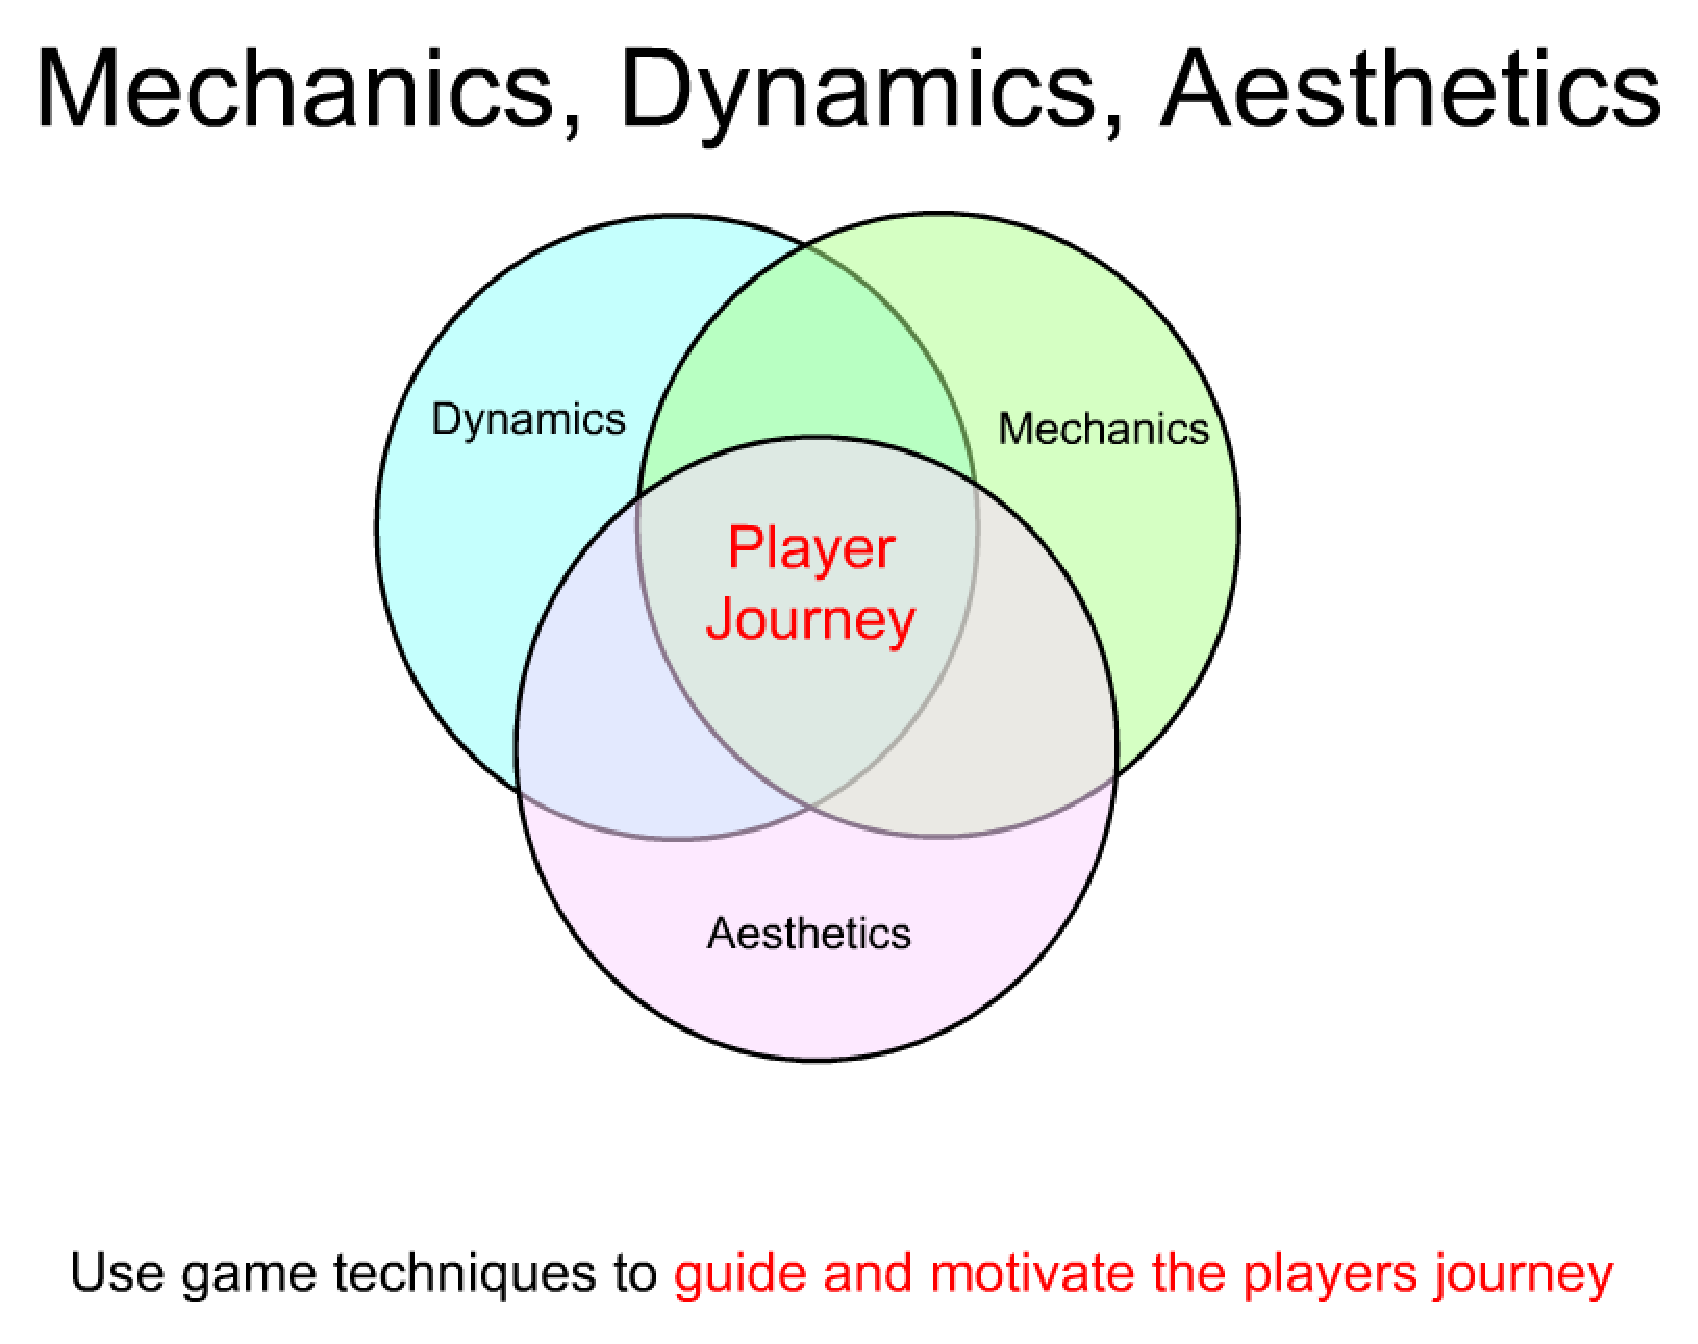
\includegraphics[height=2.1in]{kim-workshop2.eps}}
		\caption{Designing Player Journey (source: Kim \cite {Kim2010})}
		\label{fig:design-player-journey}
\end{figure}

Similarly, Sebastian Deterding not only criticized the current practice of simple gamification practices but stressed the important of ``meaningful play'' and proposed a user experience design around the three most important aspects: Meaning, Master and Autonomy \cite {Deterding2011meaningful}, It is an adaptation to the three elements to motivate people in Daniel Pink's book ``Drive: The Surprising Truth About What Motivates Us" \cite {pink2009drive}. Deterding explained that the reason why we play is because of the meaning and autonomy (choices) in the game. The mastery in the game give us fun and enjoyment.

The design of Makahiki is influenced by the above game design thinking. It combines extrinsic rewards such as prizes and achievement badges with the intrinsic motivation such as improving our environments by learning. Makahiki employs Kim's player journey idea \cite{Kim2010} to design the on-boarding and progression of levels in the smart grid game. Other game mechanics, such as the ``appointment mechanics'' and the ``social interaction'' described in SCVNGR's game dynamics play deck\cite{Biggs2010} are being used in Makahiki to improve player engagement. 

\section{Serious Game Frameworks}
\label{sec:rel-sg-framework}

Game frameworks (also known as game engines) \cite{sherrod2006ultimate} are ``comprised of a collection of different tools, utilities, and interfaces that hide the low-level details of the various tasks that make up a game''. Examples of game frameworks include:
\begin {itemize}
    \item Unreal \cite{unrealengine}:  The Unreal Engine is a game engine developed by Epic Games, it is primarily used in first person shooter games, providing tools and building blocks for 3D rendering, collision detection, AI, networking etc.
    \item PapayaMobile \cite{papayamobile}: PapayaMobile is a free cross platform social game engine on Android and iOS platform. It provides an SDK and a platform for mobile game developers to create and release games in a ``user-friendly, straightforward way''.
    \item OpenLabyrinth \cite{openlabyrinth}: OpenLabyrinth is an open source game framework that allows its users to create, run and analyze a wide range of different pathway-based activities for healthcare education.
    \item Fabula \cite{fabula}: Fabula is an open source Python game engine for adventure, role-playing and strategy games and digital interactive storytelling. It provides a library and game world abstraction intuitive to people who have not been involved in game development before and hide as much as low level technical details as much as possible.
\end {itemize}

One of the benefits of using a game framework is that, if correctly designed, it will provide useful and reusable ``building blocks'' with which to develop a variety of games. Similarly, serious game frameworks also provide building blocks that enable the serious game developer to focus more time and thought on content and results instead of on the technical details and infrastructure for creating the serious game.

There are two serious game frameworks related to sustainability development. One such framework is the Building Dashboard \cite{building-dashboard}, developed by Lucid Design Group, as shown in \autoref{fig:building-dashboard}.

\begin{figure}[ht!]
	\centering
		
\includegraphics[width=0.6\columnwidth]{building-dashboard.eps}
		\caption{Building Dashboard (source: Lucid \cite{building-dashboard})}
		\label{fig:building-dashboard}
\end{figure}

Building Dashboard is commercial platform that ``enables energy reduction competition and empowers building occupants to become active participants in energy management''. It is used to support the Campus Conservation Nationals (CCN) \cite{competetoreduce}, a nationwide electricity and water use reduction competition on college campuses. In CCN 2014, the framework was used by 109 schools in North America to display the energy and water consumption of the competition participants. It enables viewing, comparing and sharing building energy
and water use information on the web through a visual interface.

Building Dashboard is similar to Makahiki that they are both frameworks for supporting sustainability competitions, but the
cost of Building Dashboard as a commercial system creates a barrier to wider adoption. In addition, the
Building Dashboard solution focuses on providing energy information as a passive media. Besides a scoreboard, there is little interaction between participants and the system. There are less game elements other than providing a scoreboard to display the ranking of the competing teams, moreover, there is no individual points or ranking. Unlike Makahiki, Building Dashboard does not have the concept of individual registered player account, thus it does not have the capability to provide the evidence of individual player engagement.

Another framework related to sustainability is the Stanford Energy Services Platform \cite{Armel-2012}, as shown in \autoref{fig:stanford-platform}. It provides services to support the creations of energy efficiency program and research. The services include data storage, a recommendation system, user registration and participation assignment, surveys and analytics. It had been utilized to support the implementation of several of Stanford's energy saving projects and energy related serious games, such as the Power House game, Power Down game, and Energy Calculator. At this point, there is not enough information about the Stanford Energy Services Platform regarding the availability and features. 

\begin{figure}[ht!]
	\centering
		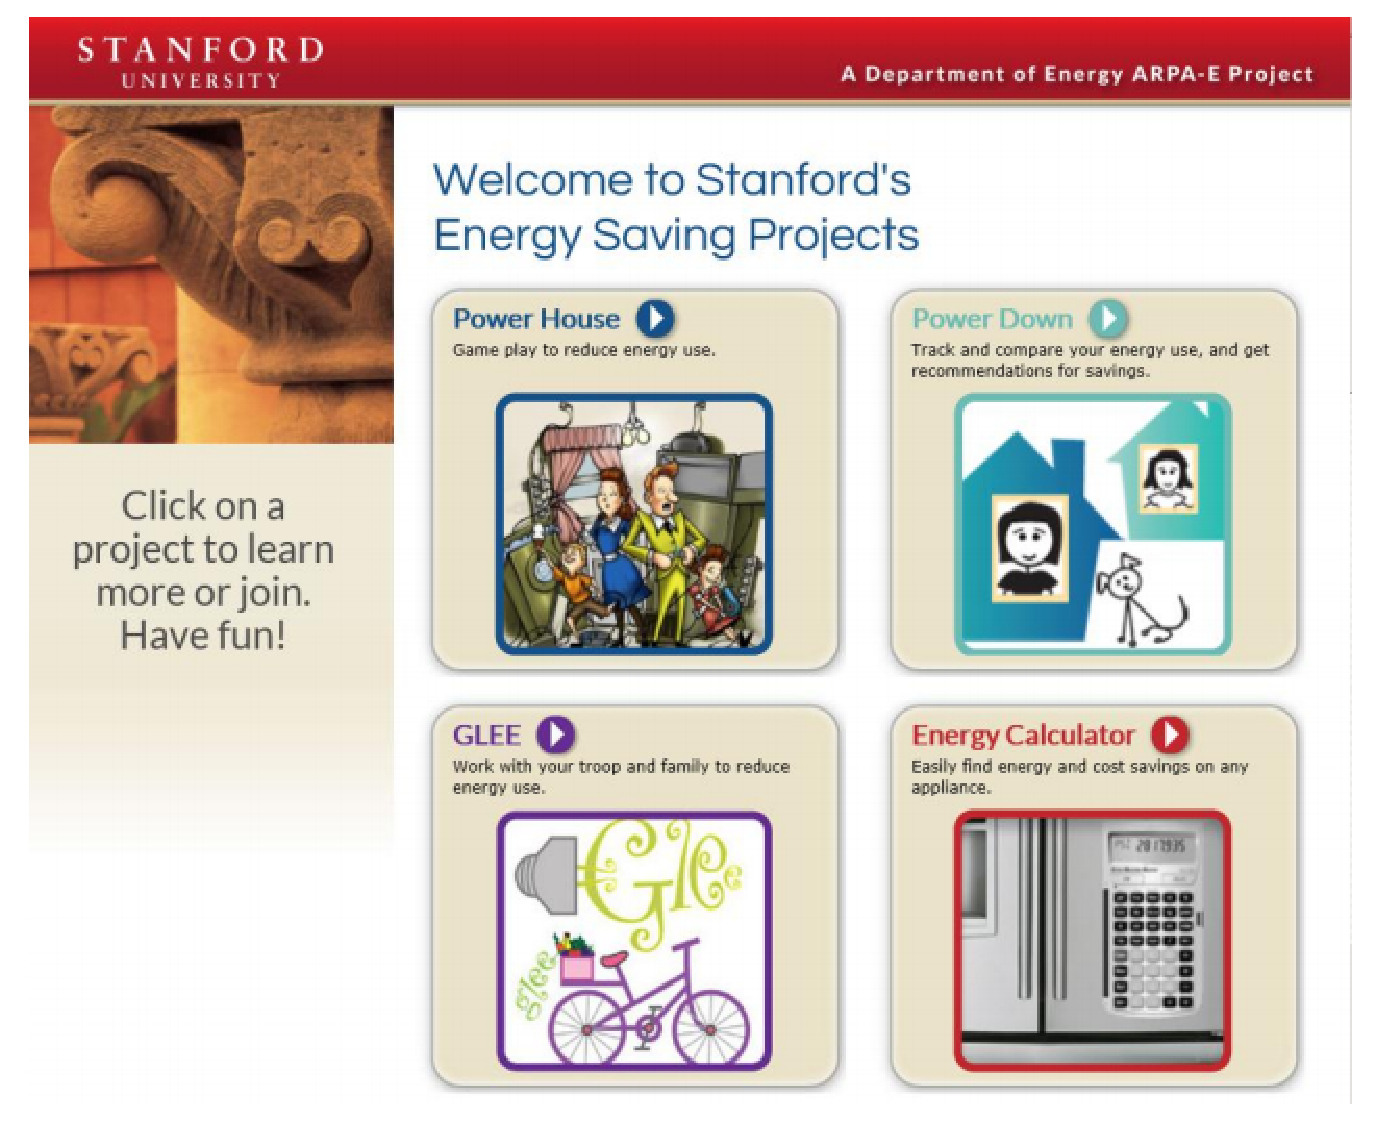
\includegraphics[width=0.6\columnwidth]{stanford-esp.eps}
		\caption{Stanford Energy Services Platform (source: Stanford \cite{Armel-2012})}
		\label{fig:stanford-platform}
\end{figure}
 
%% TODO: add non-serious game framework assessment
\section{Serious Game and Framework Assessment}
\label{sec:rel-sg-assessment}

This section examines the assessment of serious game frameworks. It starts by looking at the assessment of serious games, then  the assessment of game frameworks in general. From my literature search, I have not yet found any prior work concerning the comprehensive approach for the particular needs of a serious game framework assessment. Nevertheless the research in game and framework assessment methods provides ground works for the SGSEAM method that we designed for use in assessing a serious game framework.

\subsection{Serious Game Assessment}

In order to assess a serious game framework such as Makahiki, it is important to assess the serious games the framework produces.  One fundamental question in evaluating a serious game is the extent to which the
game achieves its ``serious'' purpose.  This is quite different from traditional entertainment games, in which evaluation focuses on usability or playability \cite{song2007new}. In the field of serious games, there is an increasing focus on the methodology of game evaluation \cite{Mayer2012233}. 

De Freitas and Oliver \cite{de2006can} point out that there are few frameworks to support the evaluation of education games. They introduce a four dimensional framework for evaluating 
educational games and simulations. The framework consists of: the context, the pedagogy, the representation, and the learner (or player). \autoref{fig:four-dimensional-framework} illustrates the evaluation framework.

\begin{figure}[ht!]
	\centering
		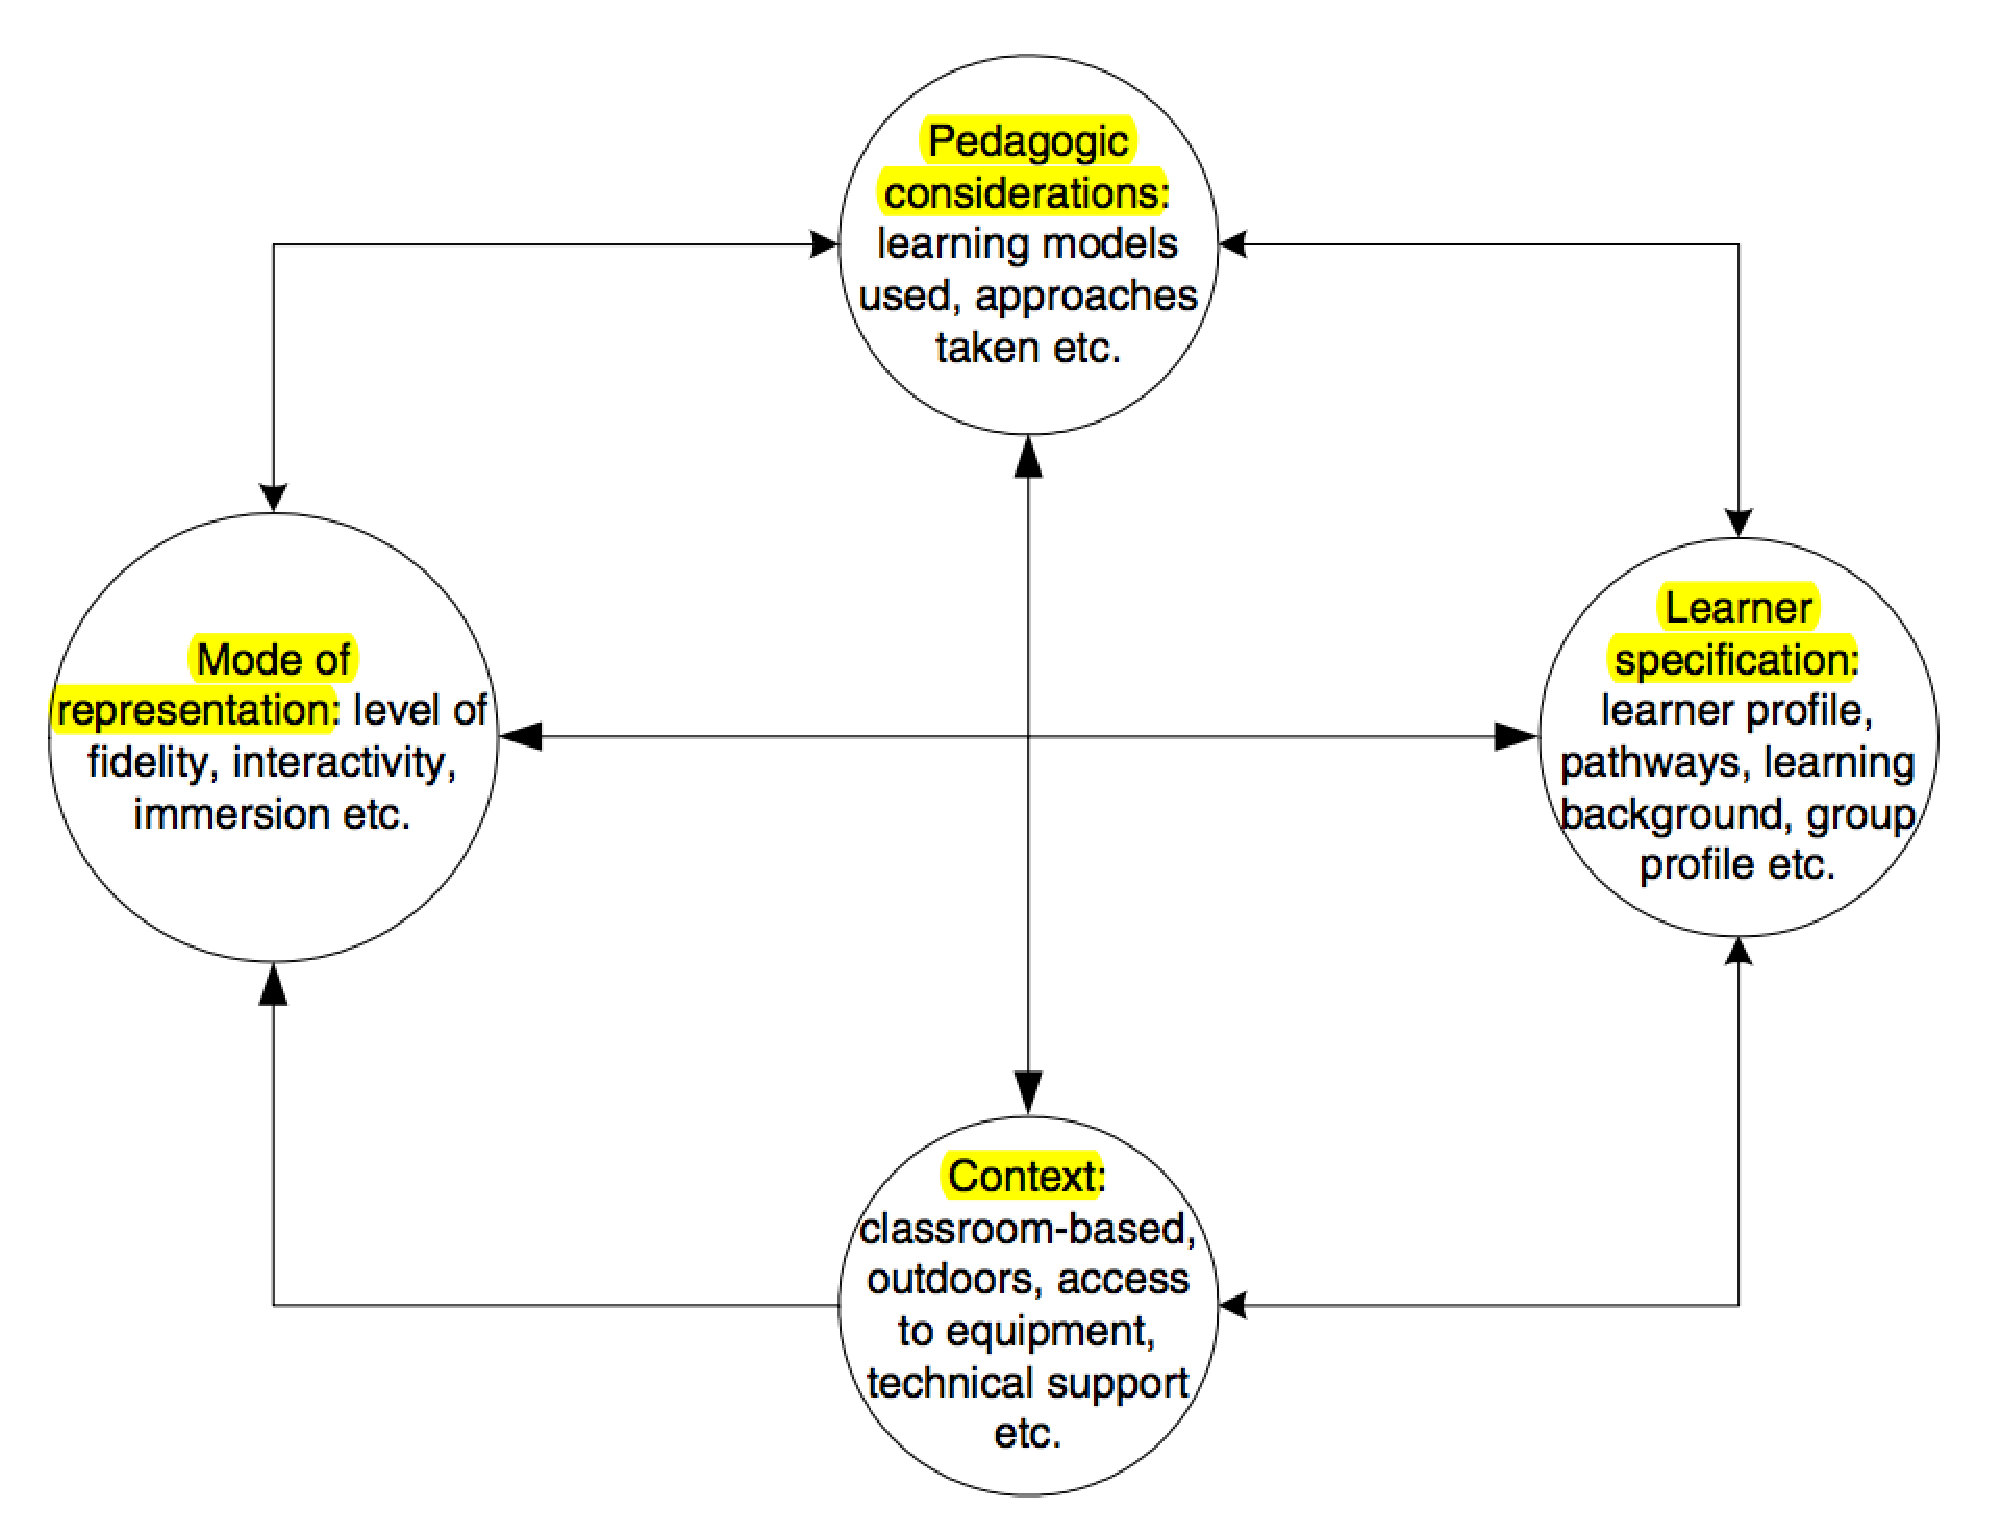
\includegraphics[width=0.6\columnwidth]{game-eval.eps}
		\caption{Four Dimensional Framework for Evaluating Educational Games \cite{de2006can}}
		\label{fig:four-dimensional-framework}
\end{figure}

Harteveld \cite{harteveld2010triadic} also agrees that ``Evaluatory research for games with a serious purpose is still at its infancy''. He proposes an evaluation framework called ``Triadic Game Evaluation (TGE)'' for assessing serious games. It consisting of three perspectives: Reality,
Meaning, and Play, as illustrated in the \autoref{fig:triadic-game-eval}.

\begin{figure}[ht!]
	\centering
		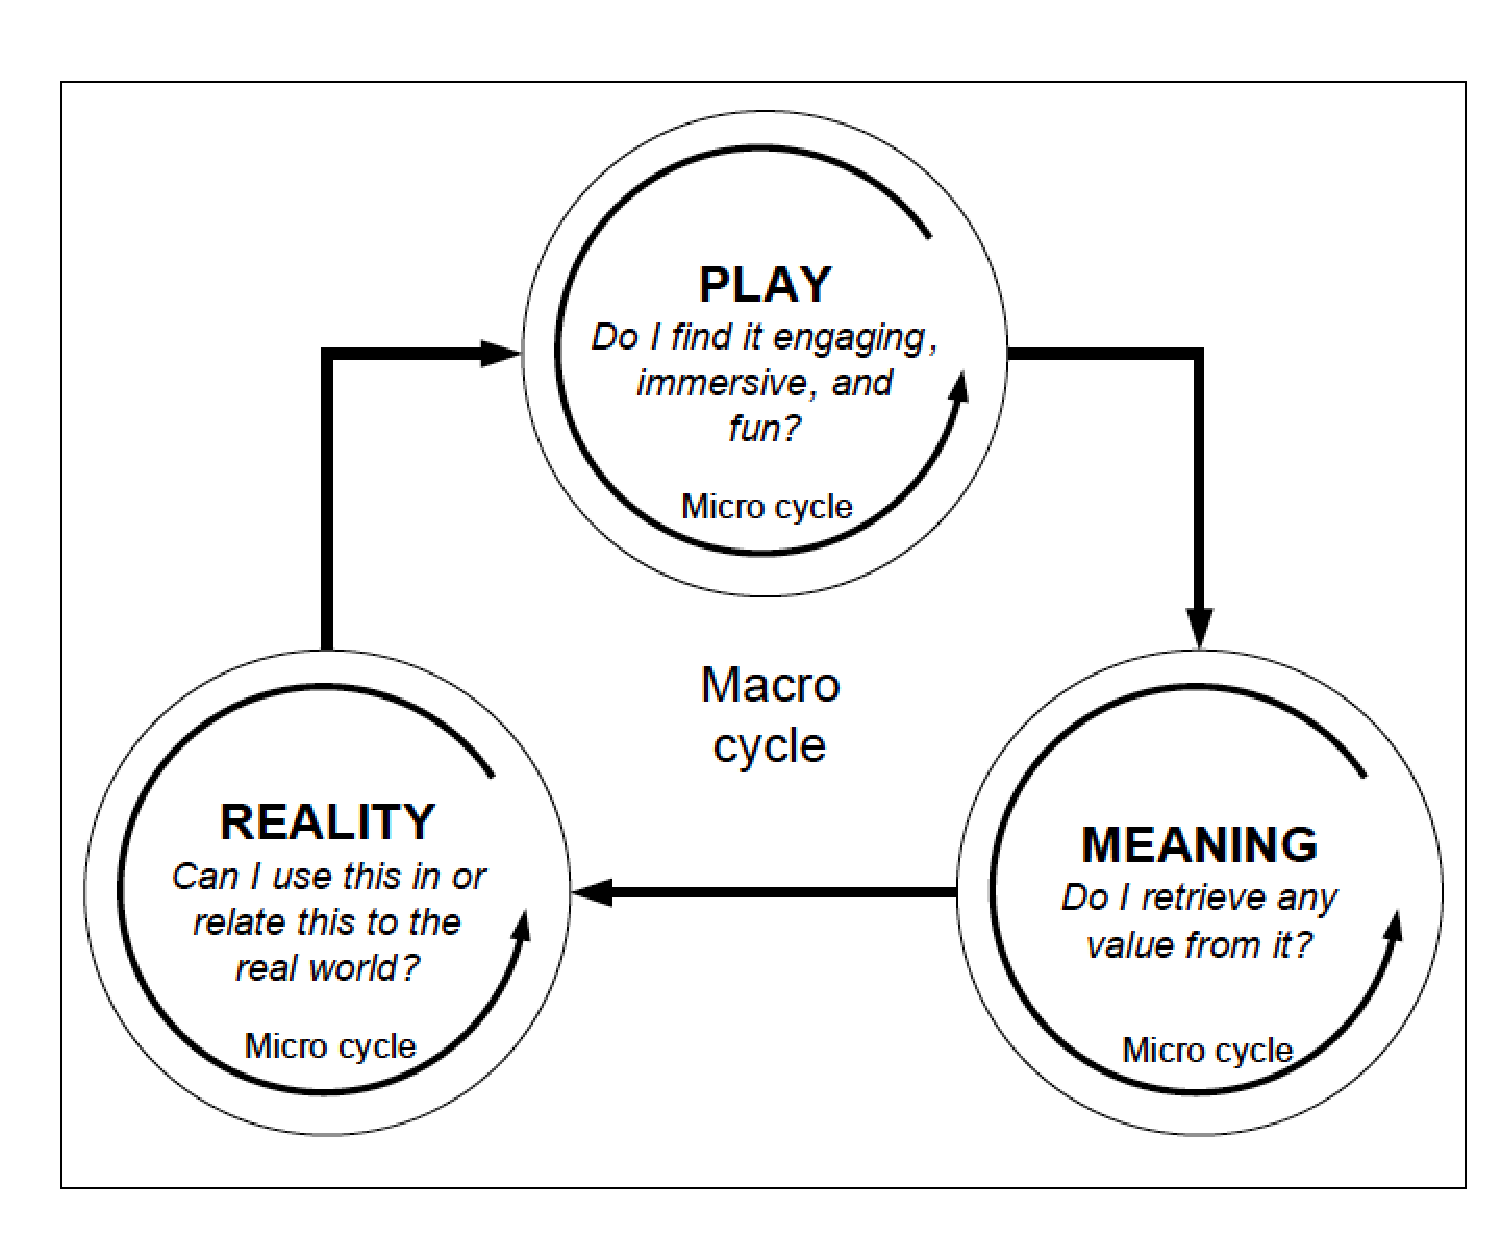
\includegraphics[width=0.6\columnwidth]{triadic-eval.eps}
		\caption{Triadic Game Evaluation (TGE) \cite{harteveld2010triadic}}
		\label{fig:triadic-game-eval}
\end{figure}

Effectiveness assessment is often part of the serious game evaluation. In their evaluation of the EnerCities game, Knol and Vries reported that they conducted a survey to test differences in awareness concerning energy-related issues between a group who had actually played the game and those who had not (between-participants design). Examples of the survey questionnaires include:
\begin{itemize}
\item What did you find out about energy saving and ``green energy'' after playing the game?
\item After playing the EnerCities game I was interested in learning more about energy saving and ``green'' energy
\item Playing the Enercities game has increased my concern about the environment
\item Playing the Enercities game made me aware of the linkages between economy, energy usage and environment
\item Playing the EnerCities game made me aware that I should lower my own energy usage
\end{itemize}

\subsection{Framework Assessment}

The above approaches focus on evaluation of a single game, as opposed to a game {\em
  framework}. One of the benefits of using a game framework is that, if correctly designed, it will provide useful and reusable ``building blocks'' with which to develop a variety of games. Yet how are we to know if a game framework has been ``correctly designed''?

Berger and Muller \cite {fabulaengine} describe their approach of using the Technology Acceptance Model (TAM) to evaluate the custom game engine Fabula \cite{fabula}. Technology Acceptance Model \cite {davis1986technology} is a well received theoretical model on assessing user acceptance of computer-based information systems, introduced by Fred Davis in his doctoral thesis in 1985. TAM considers that system use is a response that can be predicted by user motivation, which is influenced by an external stimulus of the system's features and capabilities. \autoref{fig:tam} illustrates the original Davis model. X1, X2 and X3 in the figure represent the system features.

\begin{figure}[ht!]
	\centering
		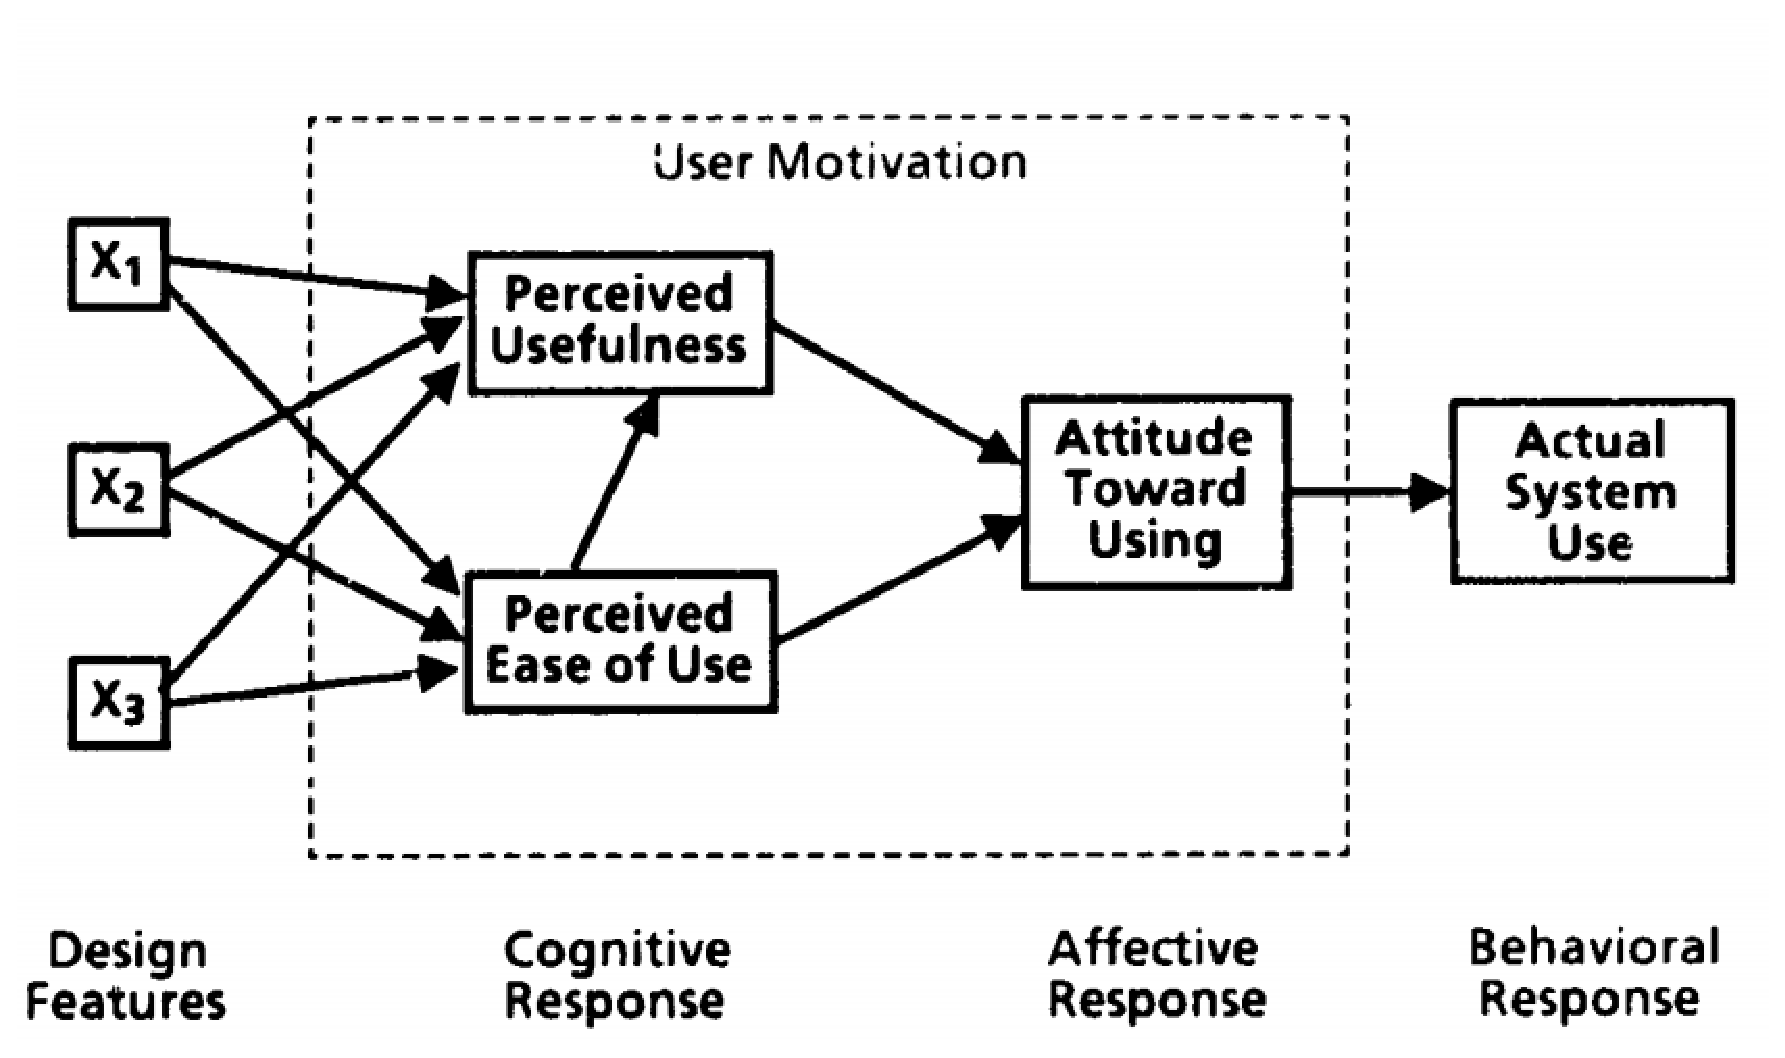
\includegraphics[width=0.6\columnwidth]{tam.eps}
		\caption{Technology Acceptance Model (TAM) \cite{davis1986technology}}
		\label{fig:tam}
\end{figure}

As Chuttur \cite{chuttur2009overview} points out in his review of TAM, there is  skepticism among some researchers regarding the rigor of the model. There exists  other assessment tools such as Game Engagement Questionnaire (GEQ) and Questionnaire for User Interaction Satisfaction (QUIS).  

Questionnaire for User Interaction Satisfaction (QUIS) \cite{harper1993improving} is a usability assessment tool developed in the HCI lab at the University Of Maryland, College Park. It is designed to assess user's subjective satisfaction regarding the human/computer interface of software systems. Currently licensing is required to access the QUIS questionnaires. 

Another usability assessment tool is the usability metrics described in Tullis and Albert 's book ``Measuring the User Experience'' \cite{tullis2010measuring}. For a usability procedure about completing transactions, Tullis and Albert suggest measuring task success, user efficiency, issues-based metrics, self-reported metrics, and live website metrics. Task success is a simple metric for a given task, does the user complete it or not? User efficiency is a measurement
of the effort required for the user to complete the task. For example, we can measure this by the amount of time spent to complete the task. Issues-based metrics involve measuring the number of times usability issues are encountered. Self-reported metrics are based on user responses to survey questions. Finally, live website metrics can be derived from analyzing the logs created by the website to understand the user experience.

\subsection{Game Metrics}

Game metrics can be as important as creativity in game design. As Nadia Oxford points out, in the game industry, player metrics collection and analysis are widely practiced to provide game designers to determine what the player audience likes and dislikes about a certain game experience \cite {Oxford2010}. 

Ducheneaut et al. provides an example of 
using game metrics to analyze player's experience in a quantitative approach \cite {ducheneaut2006alone}. They reported the relationship of playing time and leveling in the MMORGs, as shown in \autoref{fig:player-metrics}:

\begin{figure}[ht!]
	\centering
		\subfigure[Average time required to reach a level]{\label{fig:metrics1}
\includegraphics[height=1.7in]{metrics1.eps}}
		\subfigure[Average accumulated play time by level]{\label{fig:metrics2}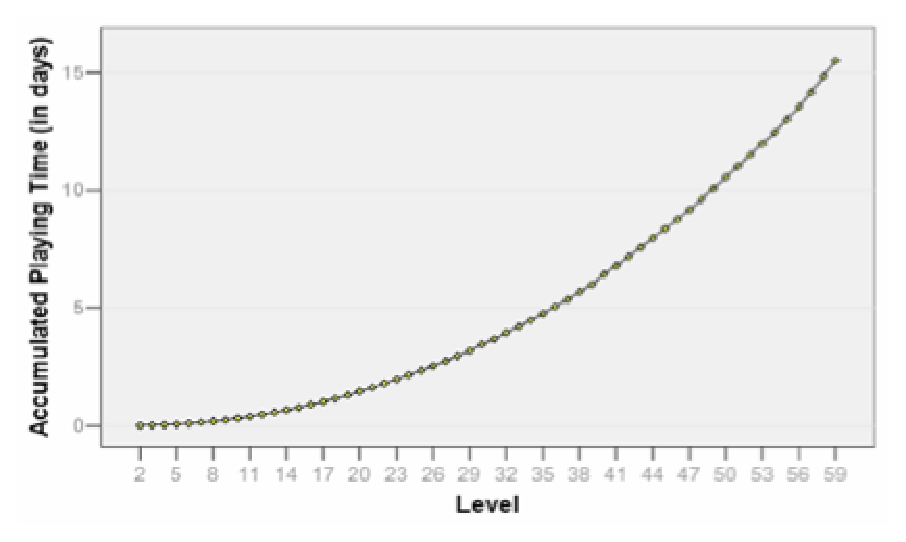
\includegraphics[height=1.7in]{metrics2.eps}}
		\caption{Player Metrics (source: Ducheneaut \cite{ducheneaut2006alone})}
		\label{fig:player-metrics}
\end{figure}

Matt Fairchild \cite {Fairchild2010} and Kontagent \cite {Kontagent2010} lists and explains some of the social games metrics as shown in \autoref{table:social-game-metrics}.

\begin{table}[ht!]
  \centering
  \begin{tabular} {|c|p{0.7\linewidth}|}
    \hline
    \tabhead{Metrics} & \tabhead{Description}\\
    \hline
	DAU & 
	Daily Active Users, is the number of active users over the course of a single day. \\
   \hline
	MAU & 
	Monthly Active Users, is the total number of users in a given month. \\
    \hline
	DAU/MAU ratio & 
	Comparing Daily Active Users to Monthly Active Users shows roughly how many days per month the average user engages with a game. \\
    \hline
	ARPU & 
	Average Revenue Per User, is measured as total revenue divided by the number of users. ARPU can be broken down by type of revenue, day, country, demographic, etc. \\
    \hline
	Churn & 
	Turnover rate (or �attrition rate�) of active players. \\
    \hline
	K Factor & 
	= (Infection Rate) * (Conversion Rate). An Infection Rate is how much a given user exposes the game to other players, such as through status updates or email invites. A conversion rate is when that ``infection'' results in a new sign up.  K factor measures the viral effect of a game. A high K Factor indicates effectiveness of bringing in new players. \\
    \hline
	Engagement &
	Measures how long users spend playing a game. How many features do they access? How many pages does the average user view? What percentage are returning visitors? \\
    \hline

  \end{tabular}
  \caption{Social Game Metrics}
  \label{table:social-game-metrics}
\end{table}

Appdata.com gathers independent application metrics from most of the social game applications. For example, the graphs in \autoref{fig:social-game-metrics} shows the DAU (Daily Active User) and MAU (Monthly Active User) metrics for the popular FarmVille \cite{farmville} social game \cite {appdata2011}:

\begin{figure}[ht!]
	\centering
		\subfigure[FarmVille DAU]{\label{fig:farmville1}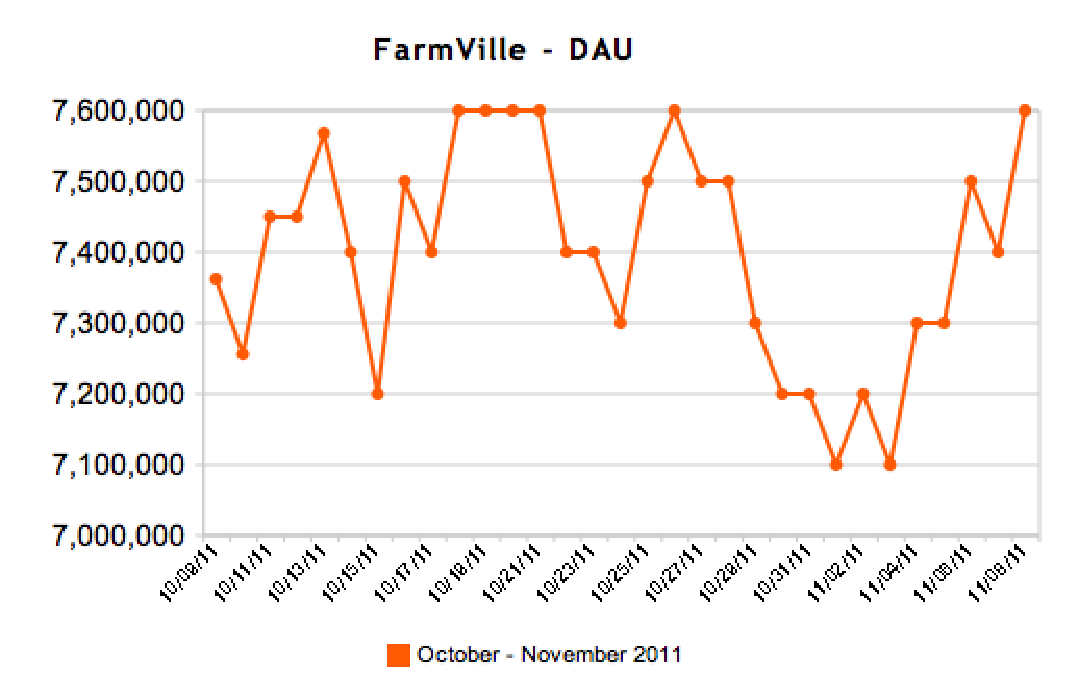
\includegraphics[height=1.85in]{FarmVille2.eps}}
		\subfigure[FarmVille MAU]{\label{fig:farmville2}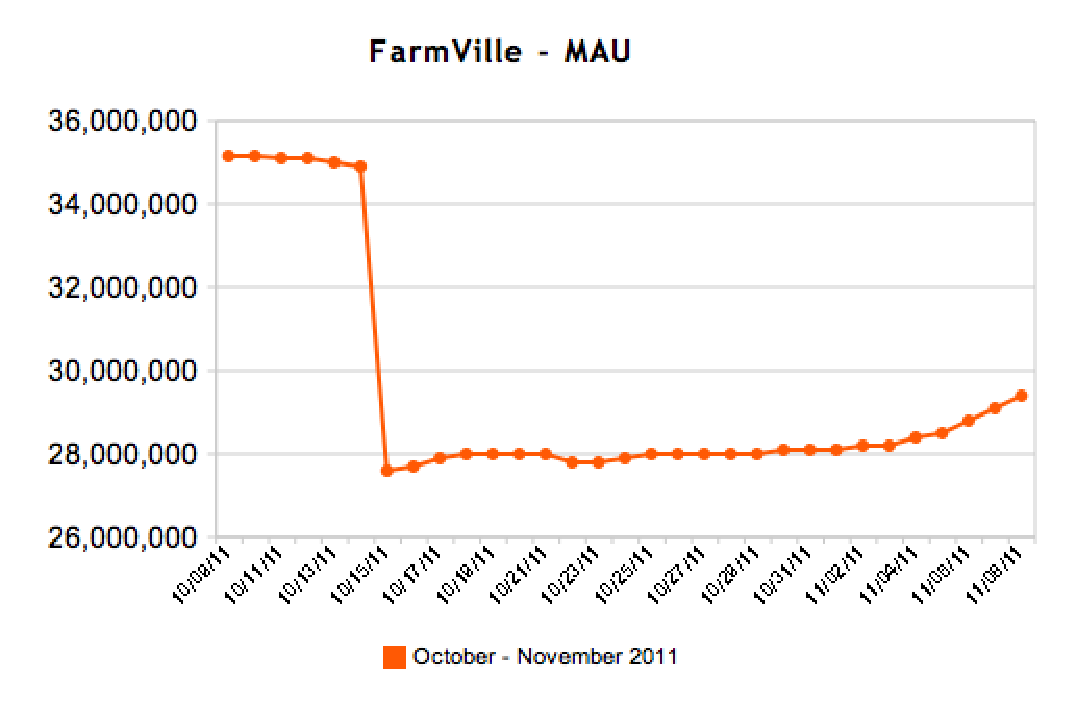
\includegraphics[height=1.85in]{FarmVille1.eps}}
		\subfigure[FarmVille DAU/MAU]{\label{fig:farmville3}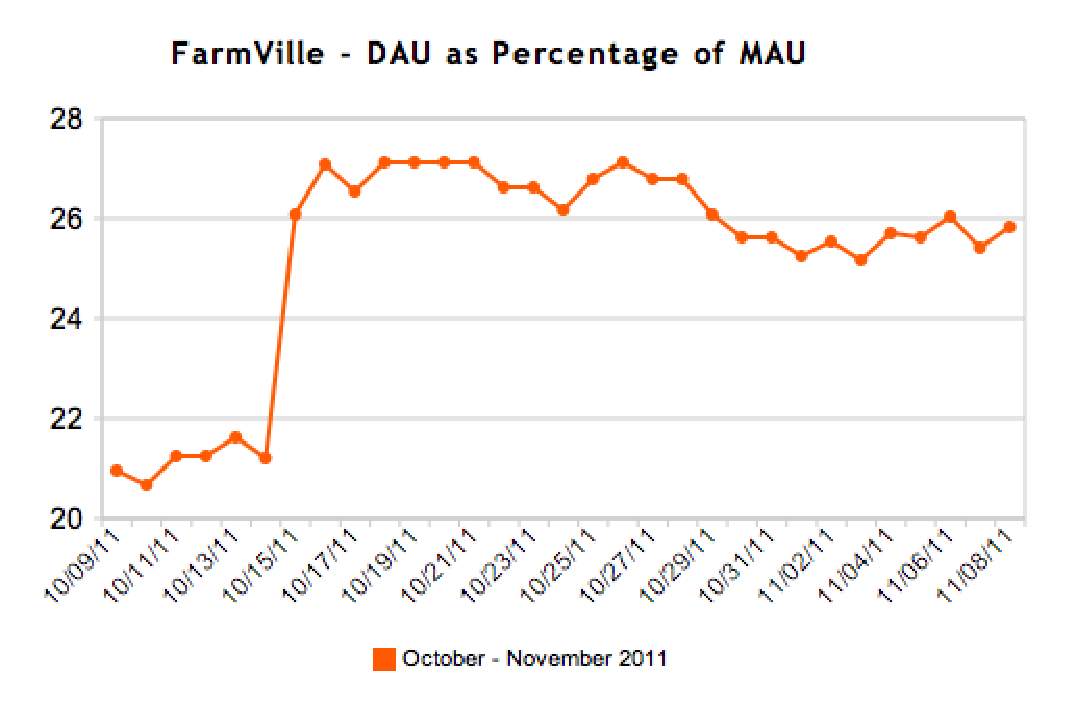
\includegraphics[height=1.85in]{FarmVille3.eps}}
		\caption{Social Game Metrics Example(source: Appdata.com \cite {appdata2011})}
		\label{fig:social-game-metrics}
\end{figure}

While the QUIS \cite{harper1993improving} is used for measuring user interaction satisfaction in a general software system, Game Engagement Questionnaire (GEQ) \cite{brockmyer2009development} developed by Brockmyer et al. is used to assess the engagement in a game. The questionnaire provides a ``psychometrically'' strong measure of levels of engagement specifically while playing video games. While the GEQ could measure the engagement level of positive game experience, the original intent of the research is to ``examine risk and protective factors for negative game impact''. \autoref{fig:geq} shows the questionnaire items.

\begin{figure}[ht!]
	\centering
		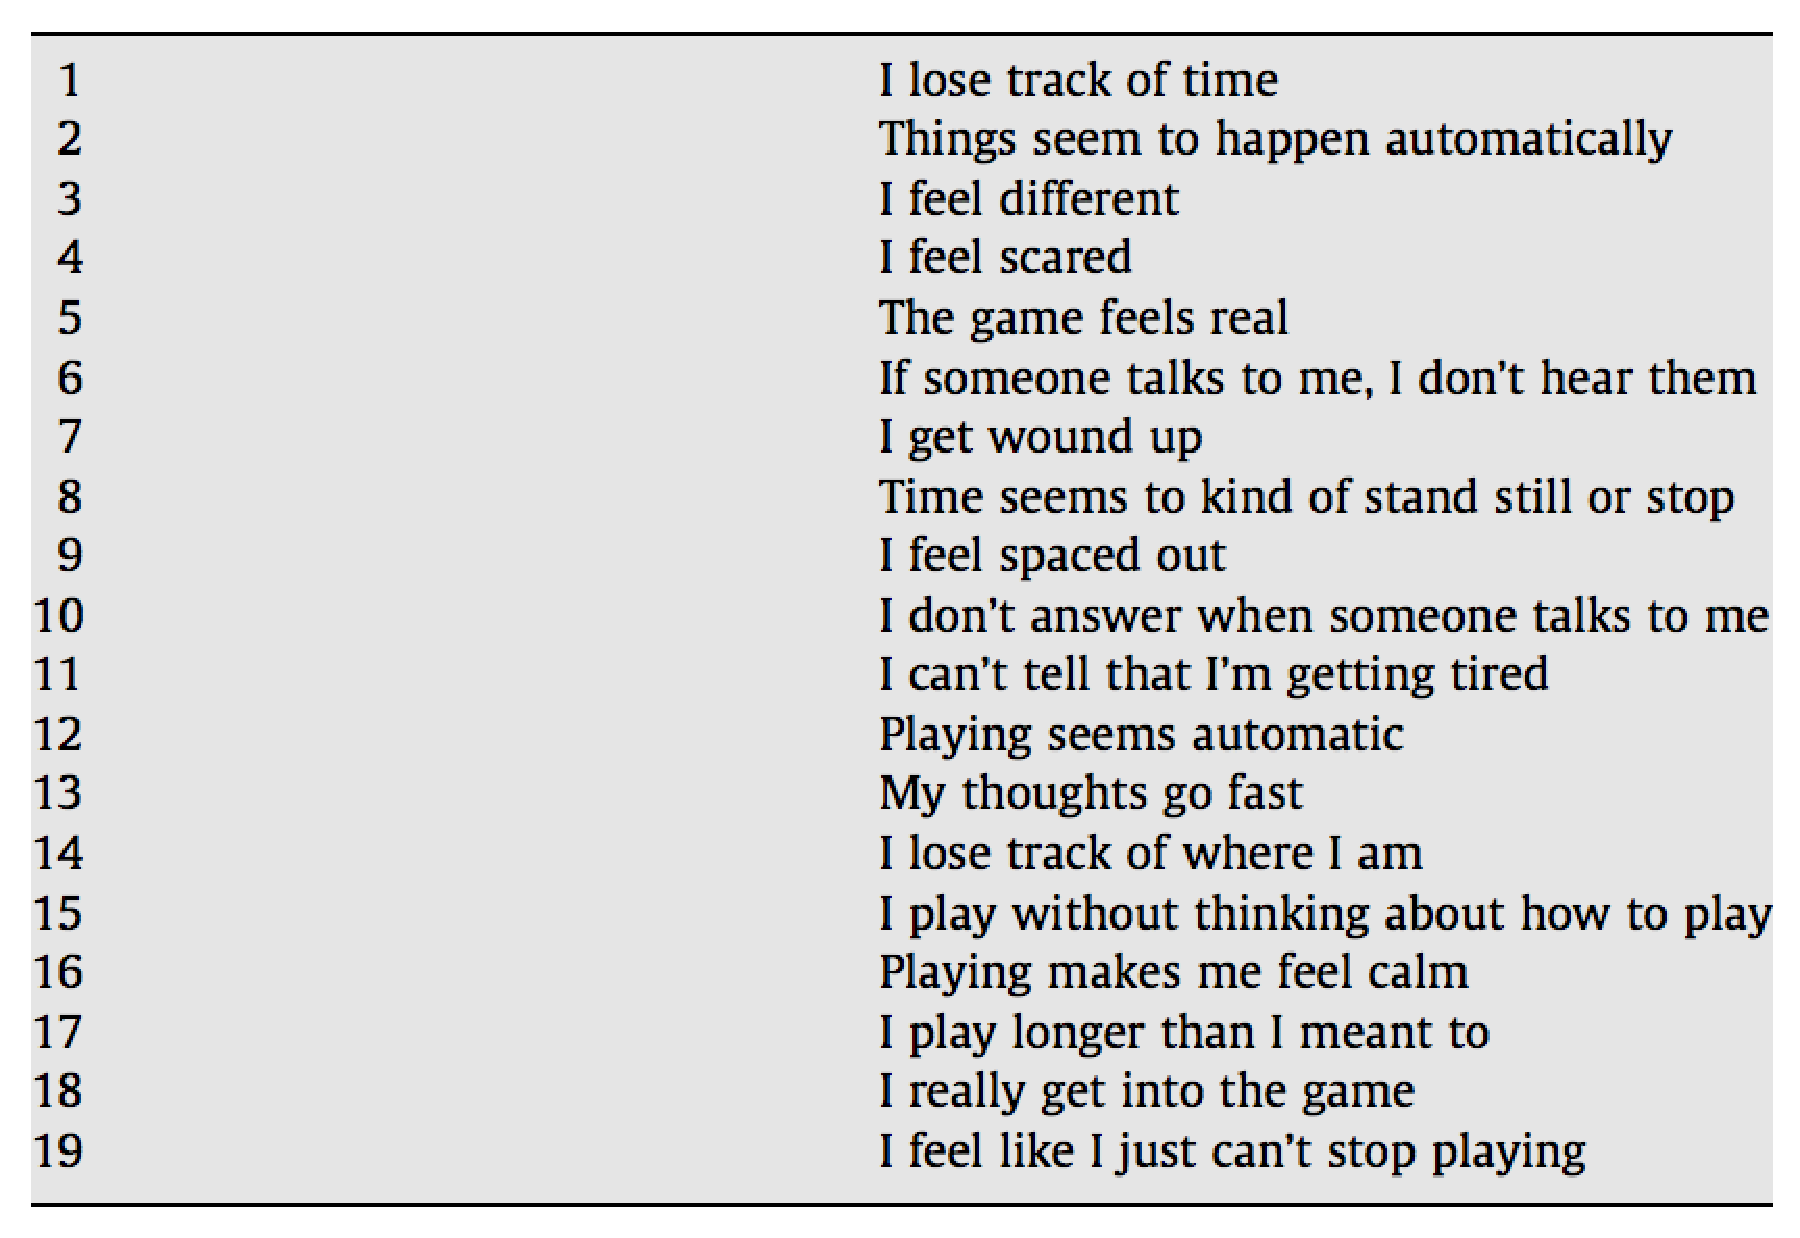
\includegraphics[width=0.7\columnwidth]{geq.eps}
		\caption{Game Engagement Questionnaire (GEQ) items \cite{brockmyer2009development}}
		\label{fig:geq}
\end{figure}

\section{Summary}
\label{sec:rel-summary}

In summary, this chapter discusses related work on serious games and gamification, game design thinking, serious games for sustainability, serious game framework and its assessment. The motivation of  Makahiki is to provide a low cost alternative to the IT infrastructure that enables the creation and managing of collegiate sustainability competitions. The design of Makahiki is inspired by the current research in game design in the context of both serious games and gamification. Serious game evaluation is an emerging field. There exists several assessment methods for serious games and for general purpose such as system usability. During my literature search, I have not found any research in the area of assessment method for serious game framework. The design of SGSEAM is to provide an assessment method for the particular needs of assessing a serious game framework.